\section{Process Models}
%Providing process models is not enough because the process owner is diffident with any result which he/she is simply provided with. Therefore, he/she wants evidence of the goodness of these models. For this purpose, you should perform alignment-based conformance checking. Using the result of the conformance checker, you should motivate why the chosen models are better that any possible alternative (e.g. because of mediating fitness, precision, generalization and simplicity). For each model, also provide its textual description. 

\subsection{Exploring process}

For exploring a good model of a data set I first filtered the data with the (\textbf{Filter log on event attribute names}) tool for extracting the required. Then I used \textbf{Interactive data heuristic miner} and \textbf{Inductive Miner} on the filtered data set to discover different models. After comparing the outcomes I decided to concentrate on \textbf{Interactive data heuristic miner} and their directly followed graphs and petri nets for understanding the lifecycle. I think the petri net is the best with basic configuration and just different frequency filters. The conformance checking where done with \textbf{Replay a log on Petri Net for conformance analysis} tool on the petri net and the filtered data. For the precision check I applied the \textbf{Multi-perspective Process Explorer} tool on the petri net and the filtered data and chose "show precision mode" in the tool with basic configuration.

\subsection{Application data set}
%filter on event names
%interactive data heuristic miner oder inductive minder und dann petri net
%conformance 
%multi-perspective
Just the events beginning with "App\_..." are required. The resulting data set is saved as "Filtered App".

\subsubsection{General details of the data set}

The data set is collected between 1st of 0ct 2011 (saturday), 00:38:44 and 14th of Mar 2012 (Wednesday), 15:33:57. It contains 13087 cases with 60849 executed events.

10 different events appear: "App\_Fully\_Submission" (21.507\%), "App\_Incomplete\_Submission" (21.507\%), "App\_Rejection" (12.547\%), "App\_Pre\_Acceptation" (12.107\%), "App\_Acceptation" (8.403\%), ("App\_Finalization" (8.242\%), "App\_Cancellation" (4.613\%), "App\_Initiation" (3.691\%), "App\_Approving" (3.691\%) and "App\_Registration" (3.691\%). Just "APP\_Fully\_Submission" appears to be a start event. However there are 8 end events possible: "App\_Rejection" (58.34\%), "App\_Cancellation" (21.449\%), "App\_Initiation" (8.573\%), "App\_Registration" (6.014\%), "App\_Approving" (2.575\%), "App\_Finalization" (2.499\%), "App\_Pre\_Acceptation" (0.527\%) and "App\_Acceptation" (0.023\%).

A trace contains maximal 8 different events and minimal 3. The mean is 4.65. In total there are 17 different variants of traces. 


\begin{figure}[!htbp]
\centering
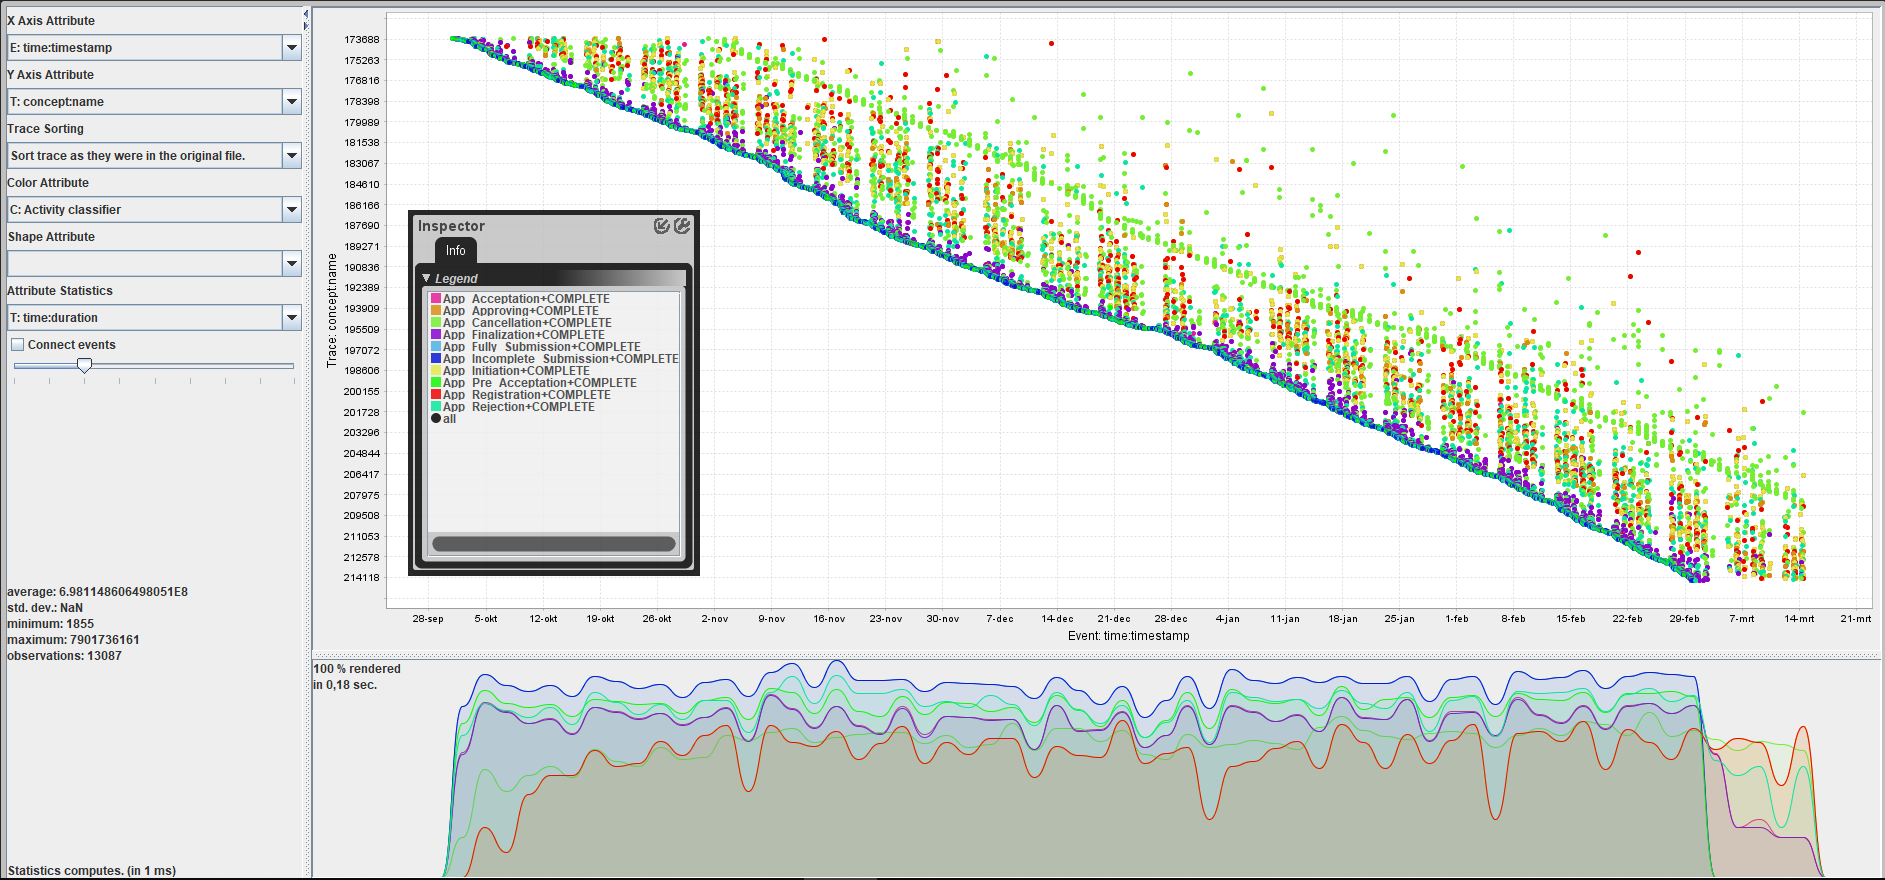
\includegraphics[height = 0.2\textheight]{AppData.PNG}
\caption{Dotted chart showing the time of events}
\label{fig:AppTimeFlow}
\end{figure}

In figure \ref{fig:AppTimeFlow} the dotted chart can be seen. Having a closer look at this chart you see gaps, which are always on a sunday. Those gaps do not appear for "APP\_Pre\_Acceptation" and "APP\_Incomplete\_Submission". Furthermore is in the left below corner to see the average duration of a case, 8 days 1 hours 55 minutes and 14.86 seconds, and the maximum duration, 91 days 10 hours 55 minutes and 36.16 seconds. Both are given in milliseconds.


\subsubsection{Discover and evaluate a model of the application lifecycle}

\begin{figure}[!htbp]
\centering
\begin{subfigure}{.4\textwidth}
  \centering
  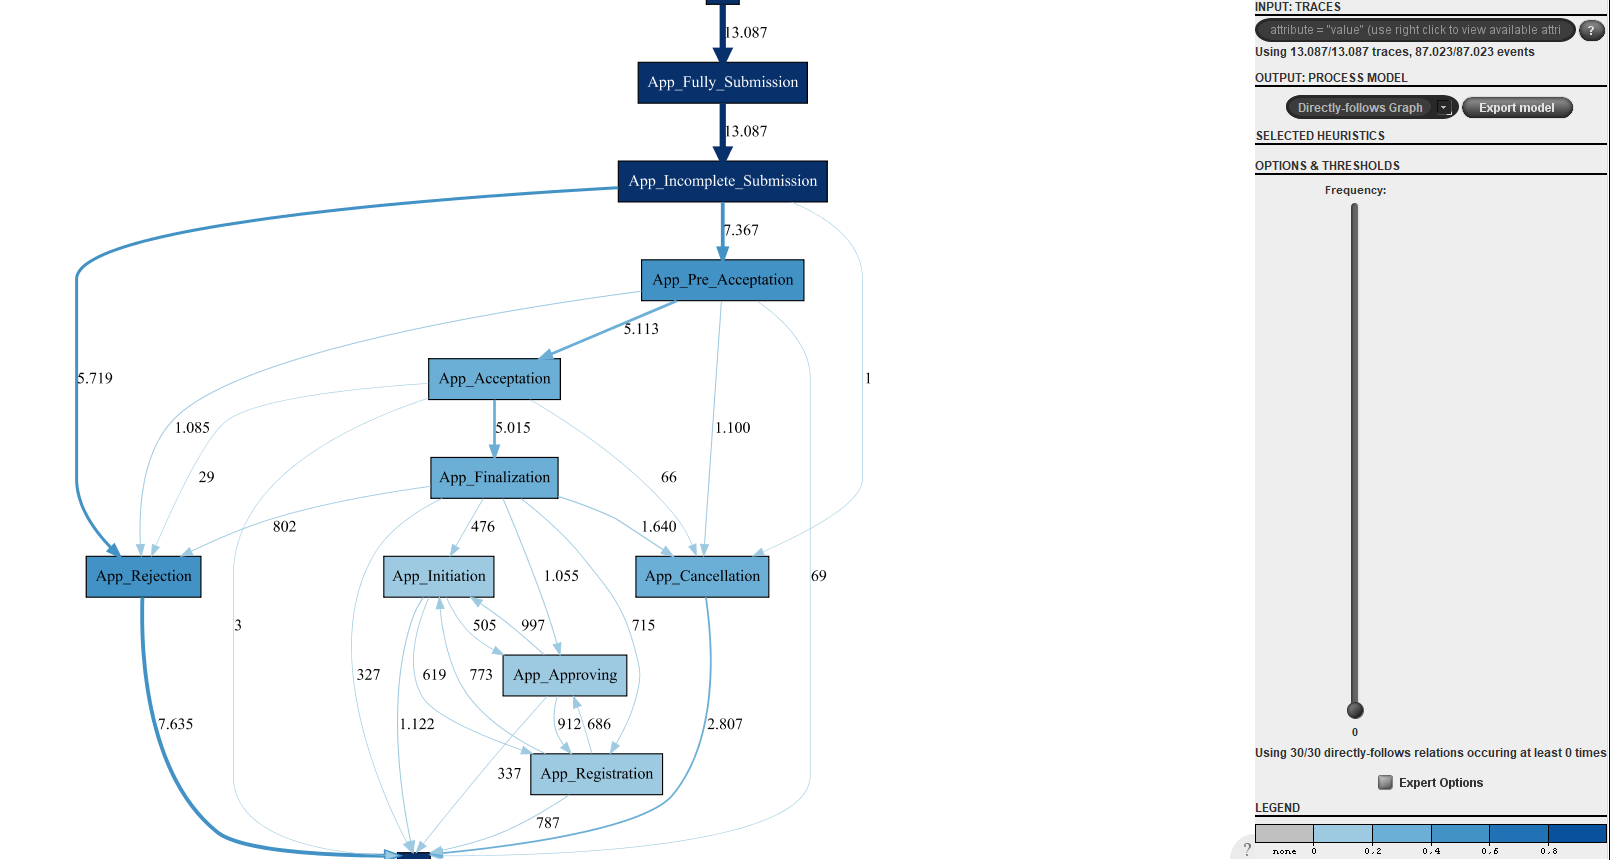
\includegraphics[width=\linewidth]{App_DirectlyFollowedFreq0.PNG}
  \caption{Petri net without frequency filtering}
  \label{fig:APP_DFG0}
\end{subfigure}%
\begin{subfigure}{.4\textwidth}
  \centering
  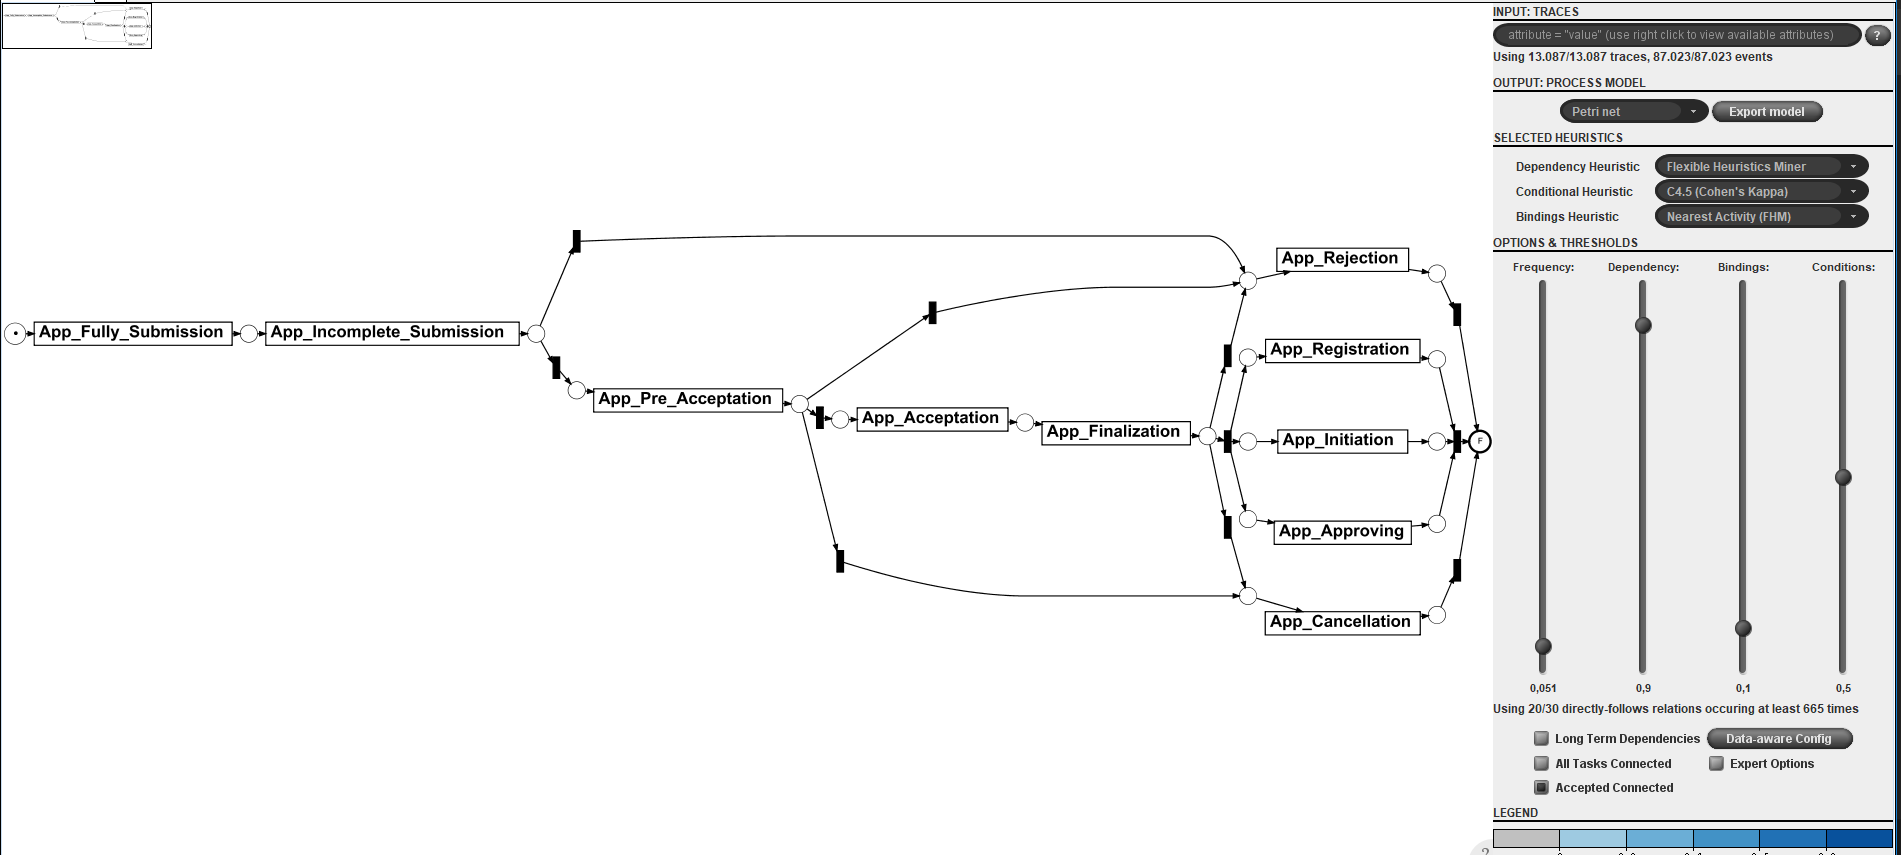
\includegraphics[width=\linewidth]{App_DirectlyFollowedFreq0-051.PNG}
  \caption{Petri net with 0.051 frequency filter}
  \label{fig:APP_DFG0-51}
\end{subfigure}
\begin{subfigure}{.4\textwidth}
  \centering
  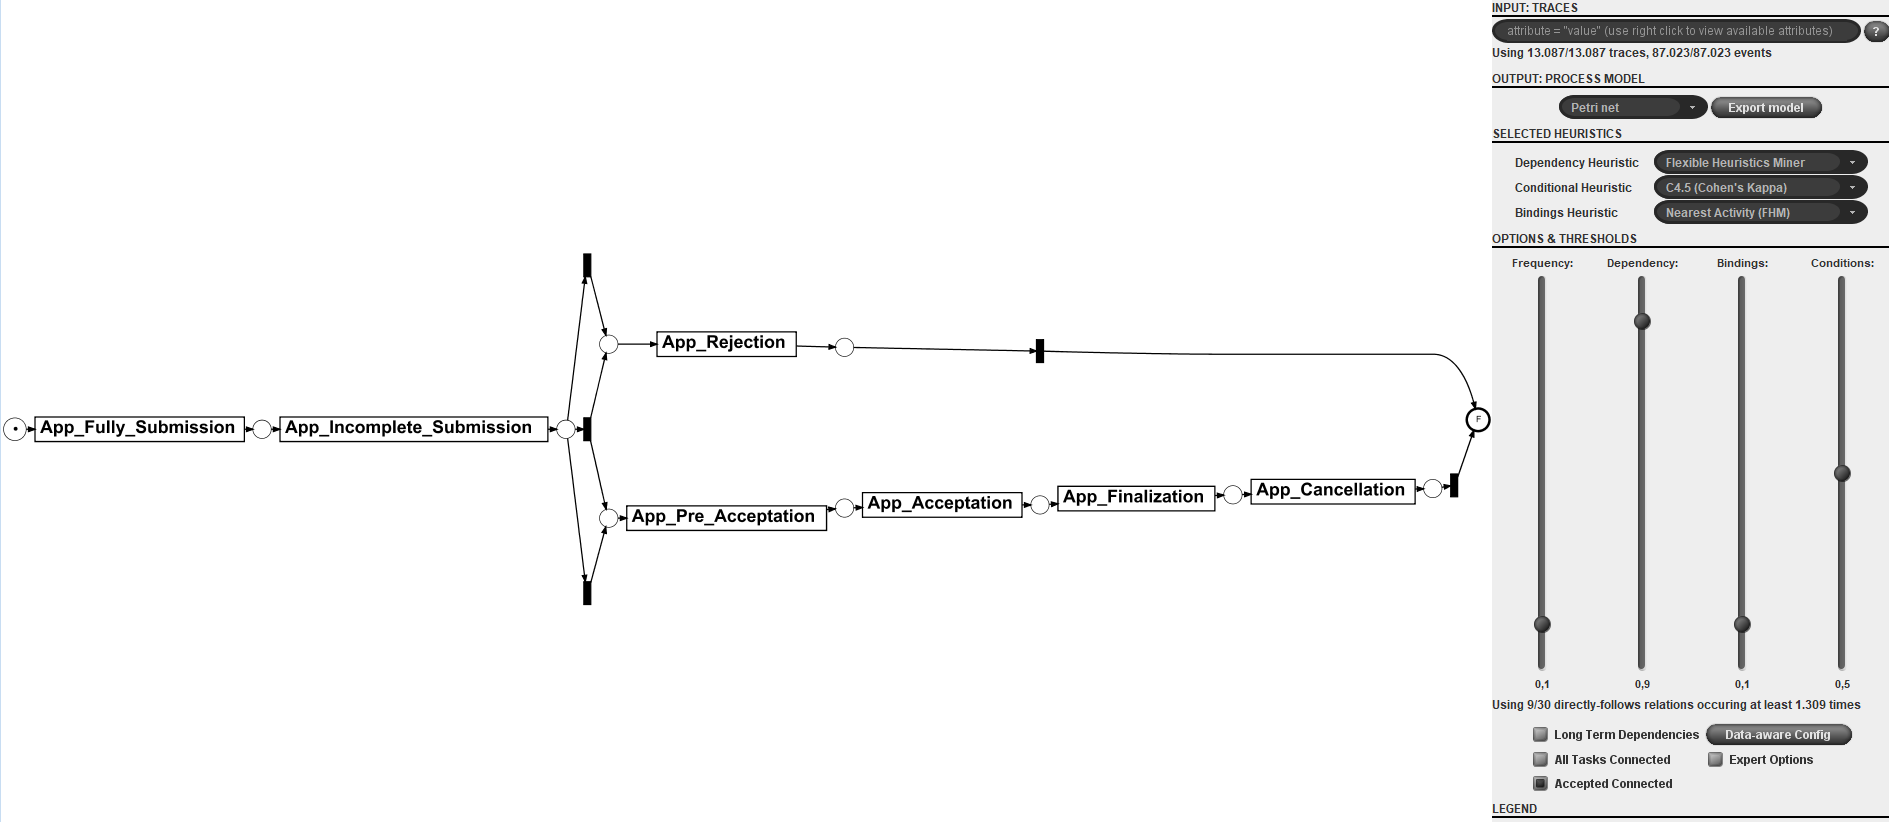
\includegraphics[width=\linewidth]{App_DirectlyFollowedFreq0-1.PNG}
  \caption{Petri net with 0.1 frequency filter}
  \label{fig:APP_DFG0-1}
\end{subfigure}
\begin{subfigure}{.4\textwidth}
  \centering
  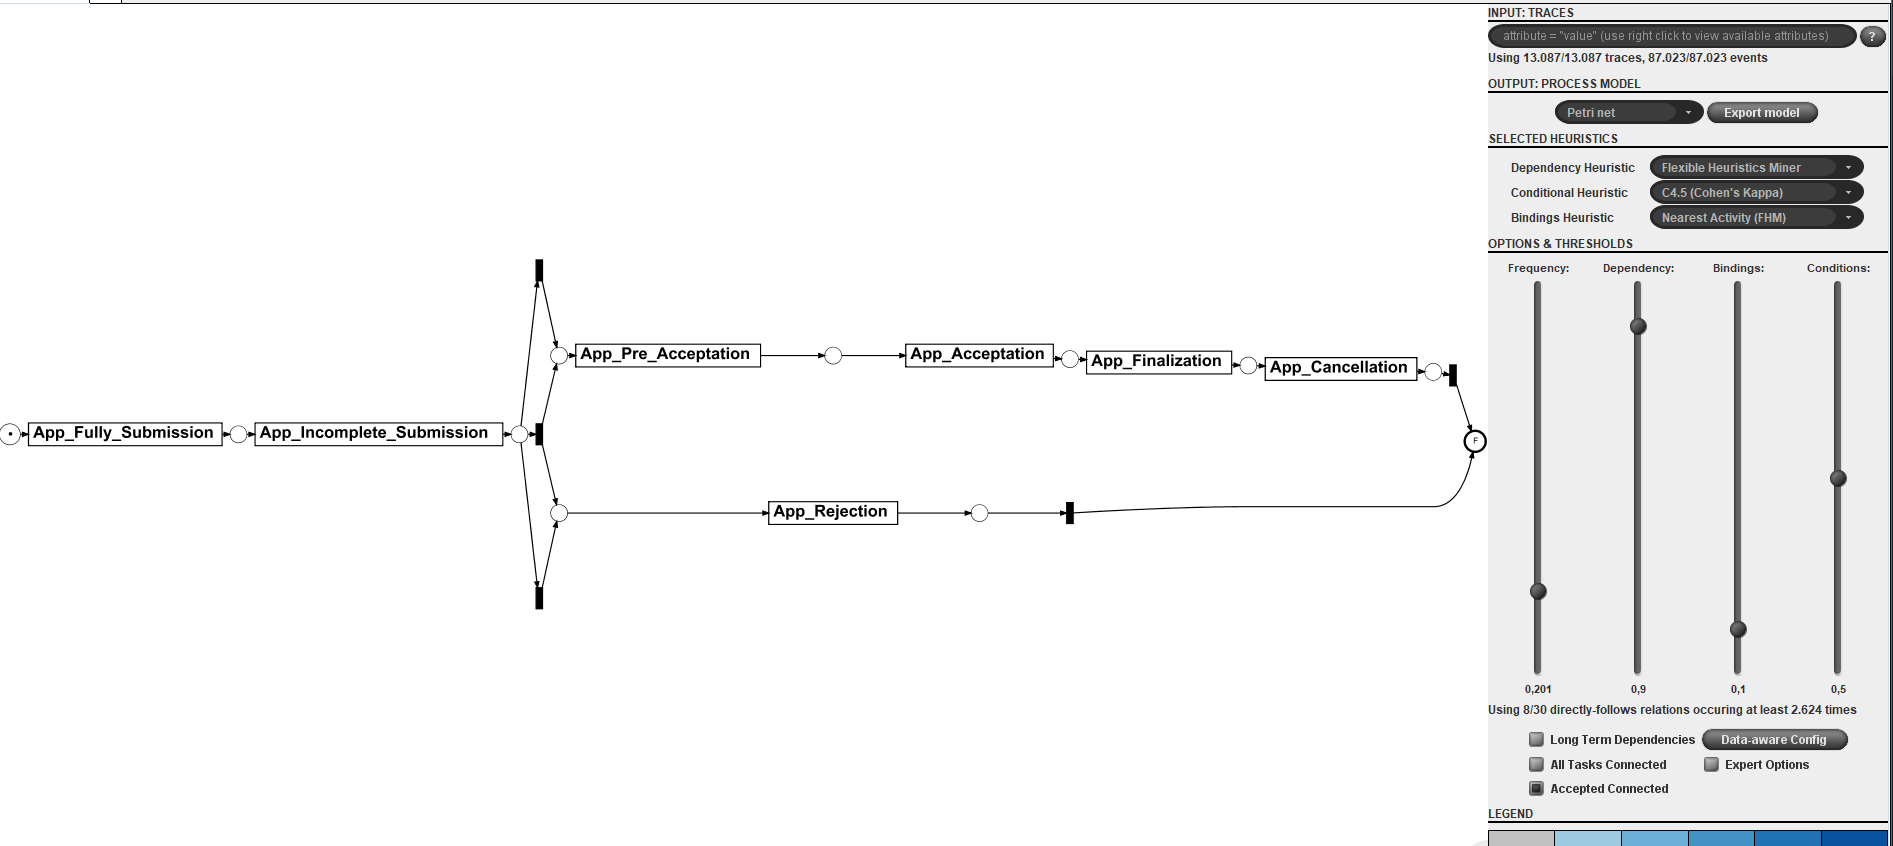
\includegraphics[width=\linewidth]{App_DirectlyFollowedFreq0-2.PNG}
  \caption{Petri net with 0.2 frequency filter}
  \label{fig:APP_DFG0-2}
\end{subfigure}
\caption{Considered petri nets}
\label{fig:App_Direct}
\end{figure}

To find an accurate model I tried different frequency filters. First I chose the frequency 0.1 and had a look at the resulting petri net. I also checked 0.2 and 0.51 for having a better understanding (not to see here is the petri net with 0.6 filtering, which was the next filtering after 0.1, that changed the net, but I decided, that it does not contain enough cases). For comparsion in the end I had also a look at the original petri net found by the \textbf{Interactive data heuristic miner}. In figure \ref{fig:App_Direct} the 4 considered petri nets can be seen. My first choice was the petri net with 0.1 as threhold for frequency, because it was a simple model that still tells us a lot about the main process (90\% of the cases) and is not to specific (still has an acceptable generalization). Obviously the original graph does not fullfill the criterium of simplicity and also the graph with frequency 0.051 still looks not as simple. I do not consider the 0.2 filtering in the next steps, because it is the same petri net as the 0.1 filtered one.

\begin{figure}[!htbp]
\centering
\begin{subfigure}{.25\textwidth}
  \centering
  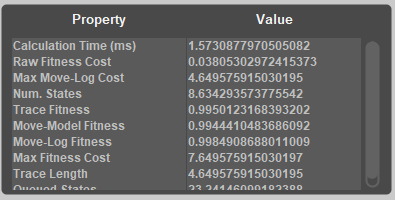
\includegraphics[width=\linewidth]{App_Conformance0-051.PNG}
  \caption{Conformance for 0.051 frequency filter}
  \label{fig:APP_Conf0-051}
\end{subfigure}%
\begin{subfigure}{.25\textwidth}
  \centering
  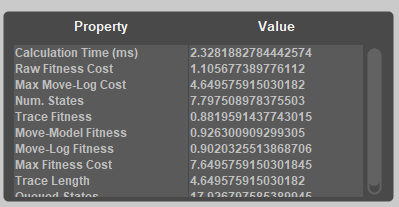
\includegraphics[width=\linewidth]{App_Conformance0-1.PNG}
  \caption{Conformance for 0.1 frequency filter}
  \label{fig:APP_Conf0-1}
\end{subfigure}
\caption{Conformance checking}
\label{fig:App_Conf}
\end{figure}


The results of the conformance checking are shown in figure \ref{fig:App_Conf}.

\begin{figure}[!htbp]
\centering
\begin{subfigure}{.4\textwidth}
  \centering
  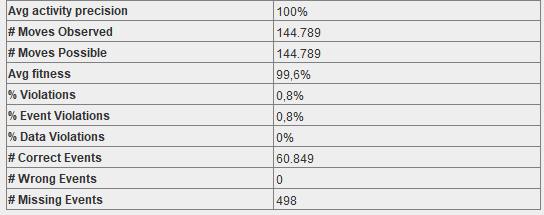
\includegraphics[width=\linewidth]{App_Precision0-051.PNG}
  \caption{Precision for 0.051 as frequency filter}
  \label{fig:APP_Prec0-051}
\end{subfigure}%
\begin{subfigure}{.4\textwidth}
  \centering
  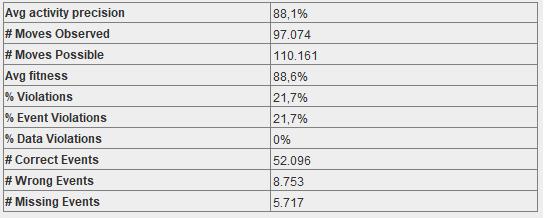
\includegraphics[width=\linewidth]{App_Precision0-1.PNG}
  \caption{Precision for 0.1 as frequency filter}
  \label{fig:APP_Prec0-1}
\end{subfigure}
\caption{Precision checking}
\label{fig:App_Prec}
\end{figure}

\begin{figure}[!htbp]
\centering
\begin{subfigure}{.9\textwidth}
  \centering
  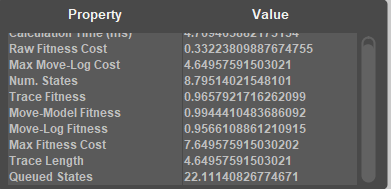
\includegraphics[width=0.4\linewidth]{App_Conformance0-069.PNG}
  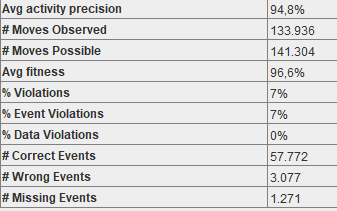
\includegraphics[width=0.4\linewidth]{App_Precision0-069.PNG}
  \caption{Conformance and Precision}
  \label{fig:APP_Conf0-069}
\end{subfigure}
\begin{subfigure}{\textwidth}
  \centering
  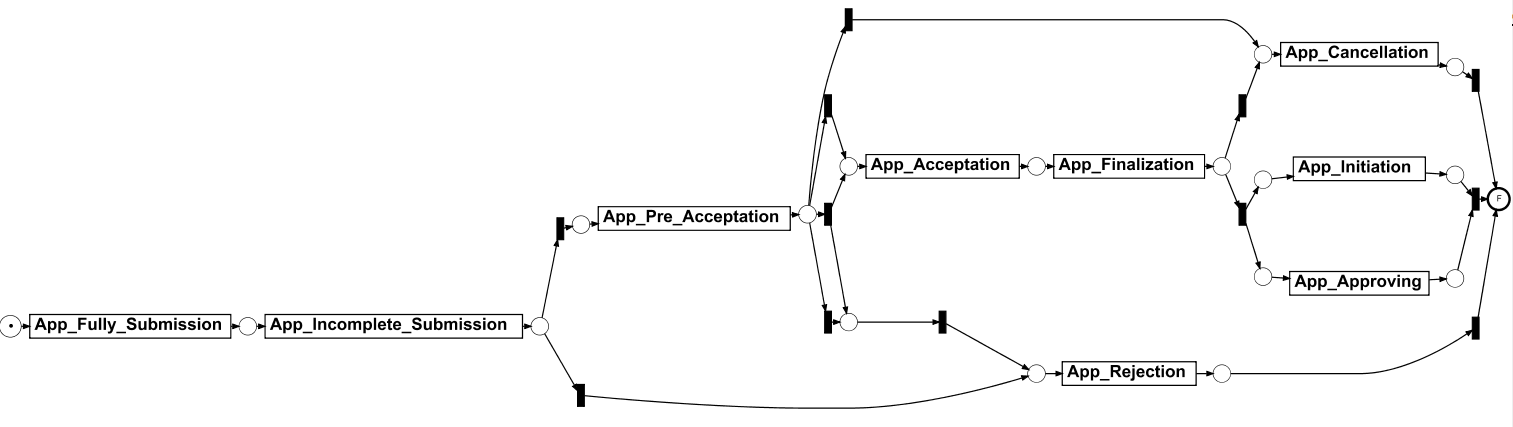
\includegraphics[width=0.9\linewidth]{App_DirectlyFollowedFreq0-069.PNG}
  \caption{Petri net}
  \label{fig:APP_DF0-069}
\end{subfigure}%
\caption{Frequency 0.069}
\label{fig:App_End}
\end{figure}
%0.07
Having a look at the precision, figure \ref{fig:App_Prec}, I could see, that the precision of 0.51 filtering is 100\%, but of the 0.1 filtering just 88.1\%. In combination with the results before, I came to the conclusion, that 0.1 filtering is not good enough as model and 0.051 would be good enough, but did not fullfill my simplicity criterium completly. Outgoing by 0.051 filtering I again tried different frequency filters starting by 0.075 to find a model fullfilling both, a similar simplicity as the 0.1 frequency model, but a better conformance and precision than this simpel model. The best result I found was with 0.069 filtering. This model is simpel enough to understand the main lifecycle, but still has good result for conformance (fitness 96.58\%) and precision(94.8\%),\ref{fig:App_End}.
Based on this I decided to choose this petri net for the lifecycle of the application data.

\subsubsection{Discussion of the lifecycle}
Simplifying the discussion I will not write "App\_.." in begin of all events, but every event mentioned in this section is from the application data set.
\begin{figure}[!htbp]
\centering
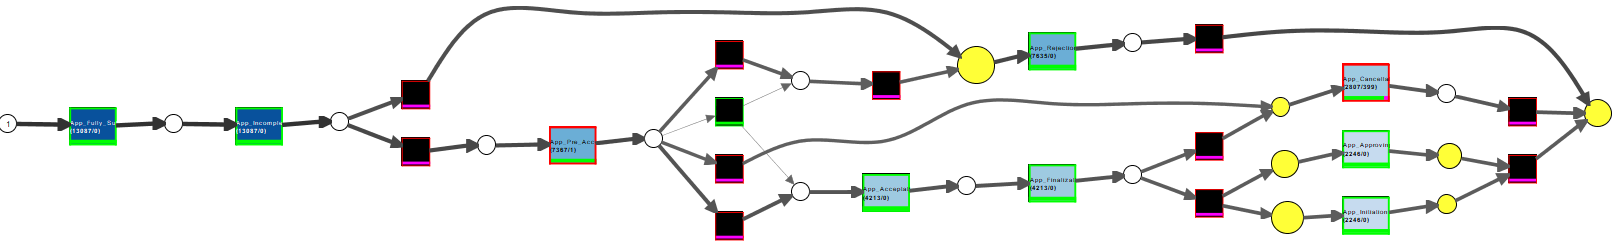
\includegraphics[width=0.9\linewidth]{APP_Replay.PNG}
\caption{Replay on petri net with 0.069 frequency filter}
\label{fig:App_EndReplay}
\end{figure}
To also have details about the occurency of the steps in the model I used the replay result, \ref{fig:App_EndReplay}.


The process always starts with "Fully\_Submission" and "Incomplete\_Submission" (13087 cases). After this there are two different outcomes:
\begin{enumerate}
	\item "Rejection" (5719 cases, executed in total in 7365 cases)
	\item "Pre\_Acceptation" (7367 cases)
\end{enumerate}

"Pre\_Acceptation" has 4 different successor events
\begin{enumerate}
	\item "Rejection" (1916 cases)
	\item "Rejection" and "Acceptation" (0 cases)
	\item "Acceptation" (4213 cases)
	\item "Cancellation" (1239 cases)
\end{enumerate}
"Acceptation" is followed by "Finalization" (4213). "Finalization" is followed in (1967 cases) by "Cancellation", which is in total executed 3206 times, and otherwise by "Approving" and Initation (2246 cases).
All the differences between incoming and outcoming cases can be explained through the filtering by frequency for building the model.

Looking at the \textbf{Time between Transition matrix} of the replay result it can be seen, that the transition to "Approving" and "Initiation" need in average \texttildelow 16 days, what is the second longest transition time. "Cancellation" has the worst transition time with in average \texttildelow 20 days.

\subsection{Proposal data}
Just the events beginning with "P\_..." are required. The resulting data set is saved as "Filtered P".

\subsubsection{General Details of the data set}
The data set is collected between 1st of 0ct 2011 (saturday), 10:44:40 and 14th of Mar 2012 (Wednesday), 15:50:59 and contains 13087 cases with 31244 events. Having a look at the visualization you can see that there a gaps in the workflow. 

\begin{figure}[!htbp]
\centering
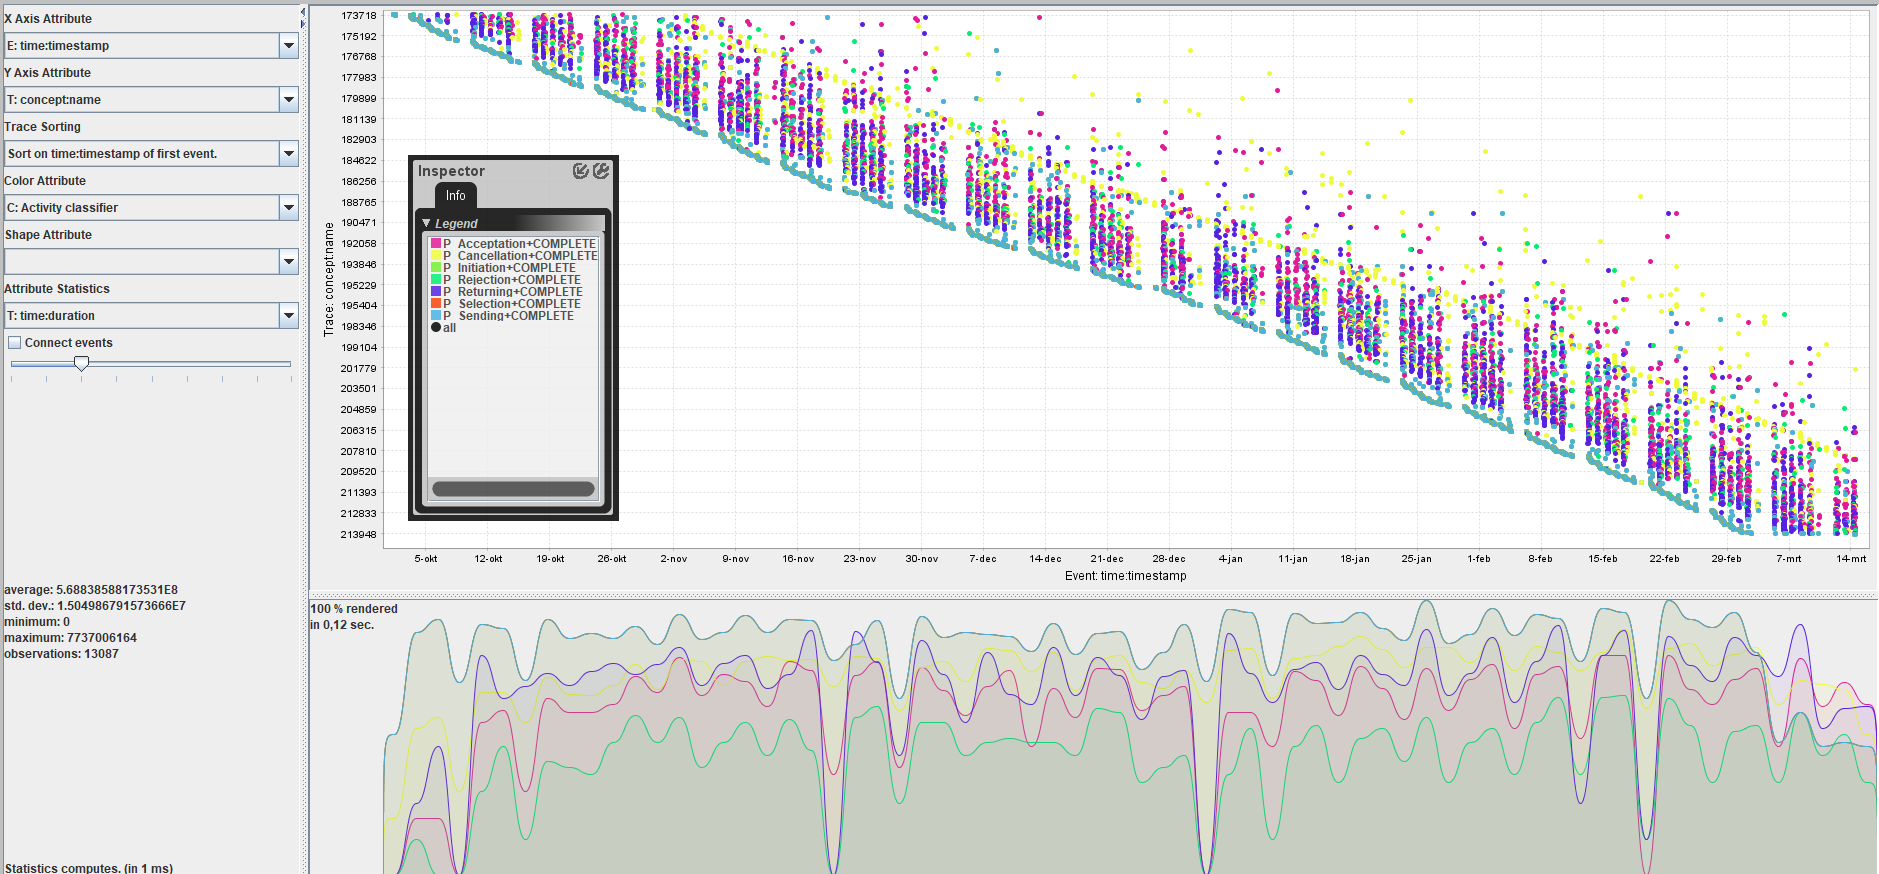
\includegraphics[height = 0.2\textheight]{ProposalData.PNG}
\caption{Dotted chart showing the time of events}
\label{fig:PropTimeFlow}
\end{figure}

In figure \ref{fig:PropTimeFlow} the dotted chart can be seen. Having a closer look at this gaps makes clear, that it is always a sunday. What does not show this behavior so clear is "P\_Cancellation" and "P\_Initiation". Furthermore is in the left below corner to see what is the average duration of a case, 6 days 14 hours 0 minutes and 38.59 seconds, and the maximum duration, 89 days 13 hours 10 minutes and 6.16 seconds. Both is given in milliseconds.

The data set has 7 events: "P\_Initiation" (22.5\%), 
"P\_Sending" (22.5\%), "P\_Selection" (22.5\%), "P\_Cancellation" (11.698\%), "P\_Returning" (11.055\%), "P\_Acceptation"(7.179\%) and "P\_Rejection" (2.567\%), where the percentage is the relative occurence. In total this data set contains 13087 cases with in total 31244 events. It always stars with "P\_Selection" and has 5 different end events: "P\_Acceptation" (44.726\%), "P\_Cancellation"(32,702\%), "P\_Rejection" (15.992\%), "P\_Sending" (4.806\%) and "P\_Returning" (1.775\%).

There are 169 different variants of traces.

Maximal 30 events are executed in a case and minimal 0, what is a hint, that there are cases ending directly. The mean of events per class is 2.387.


\subsubsection{Discover and evaluate models of the proposal lifecycle}

Applying the steps on the proposal data set it gave me 4 models I wanted to have a closer look at.

\begin{figure}[!htbp]
\centering
\begin{subfigure}{.4\textwidth}
  \centering
  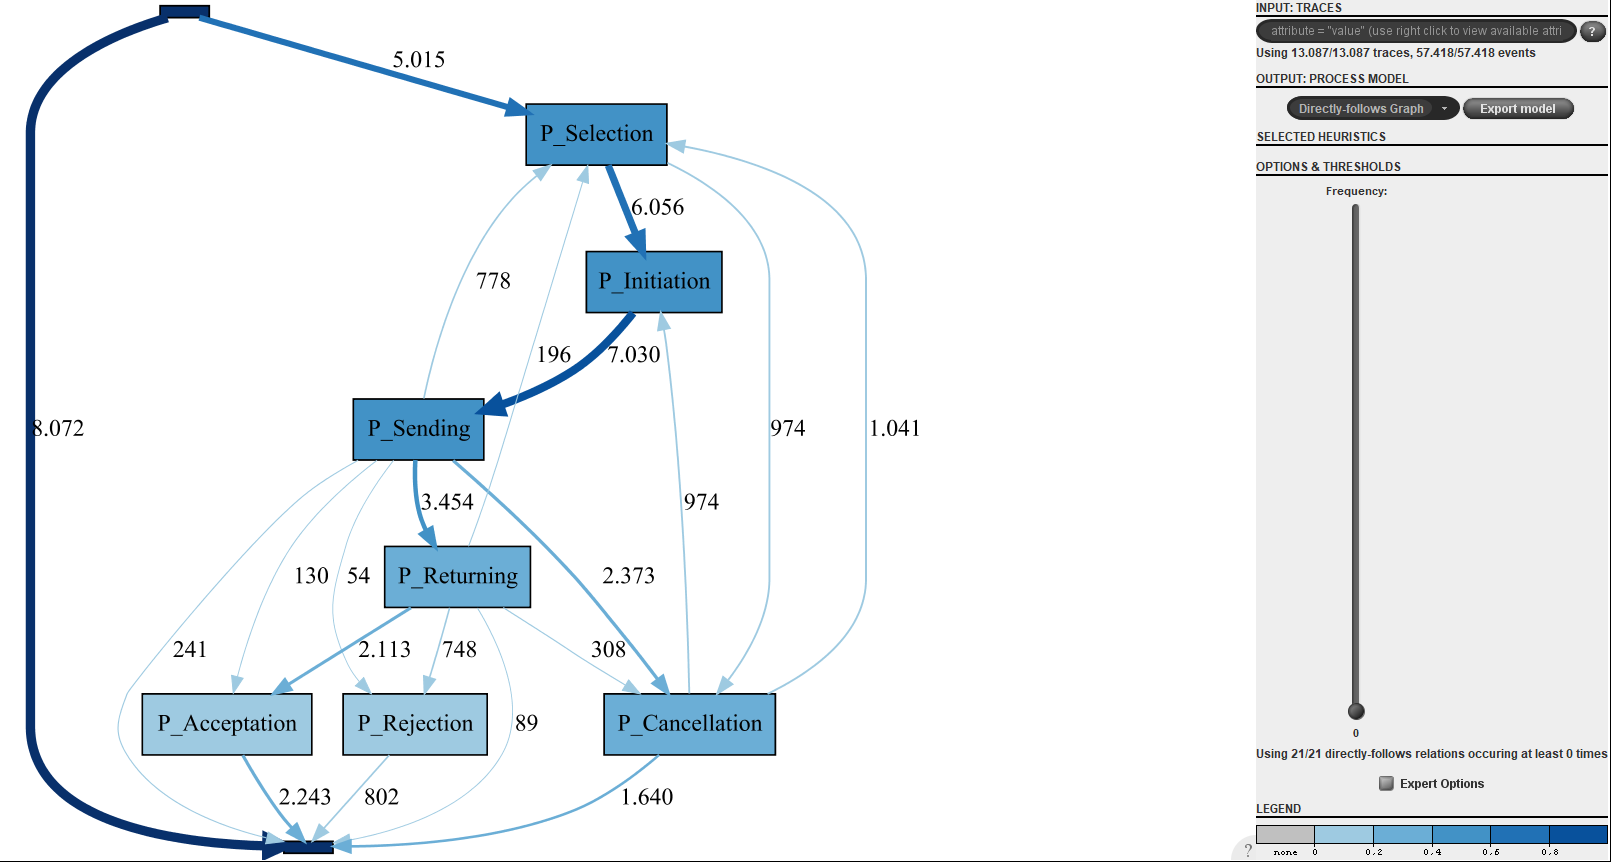
\includegraphics[width=\linewidth]{P_DirectlyFollowedFreq0.PNG}
  \caption{Petri net without frequency filtering}
  \label{fig:P_DFG0}
\end{subfigure}%
\begin{subfigure}{.4\textwidth}
  \centering
  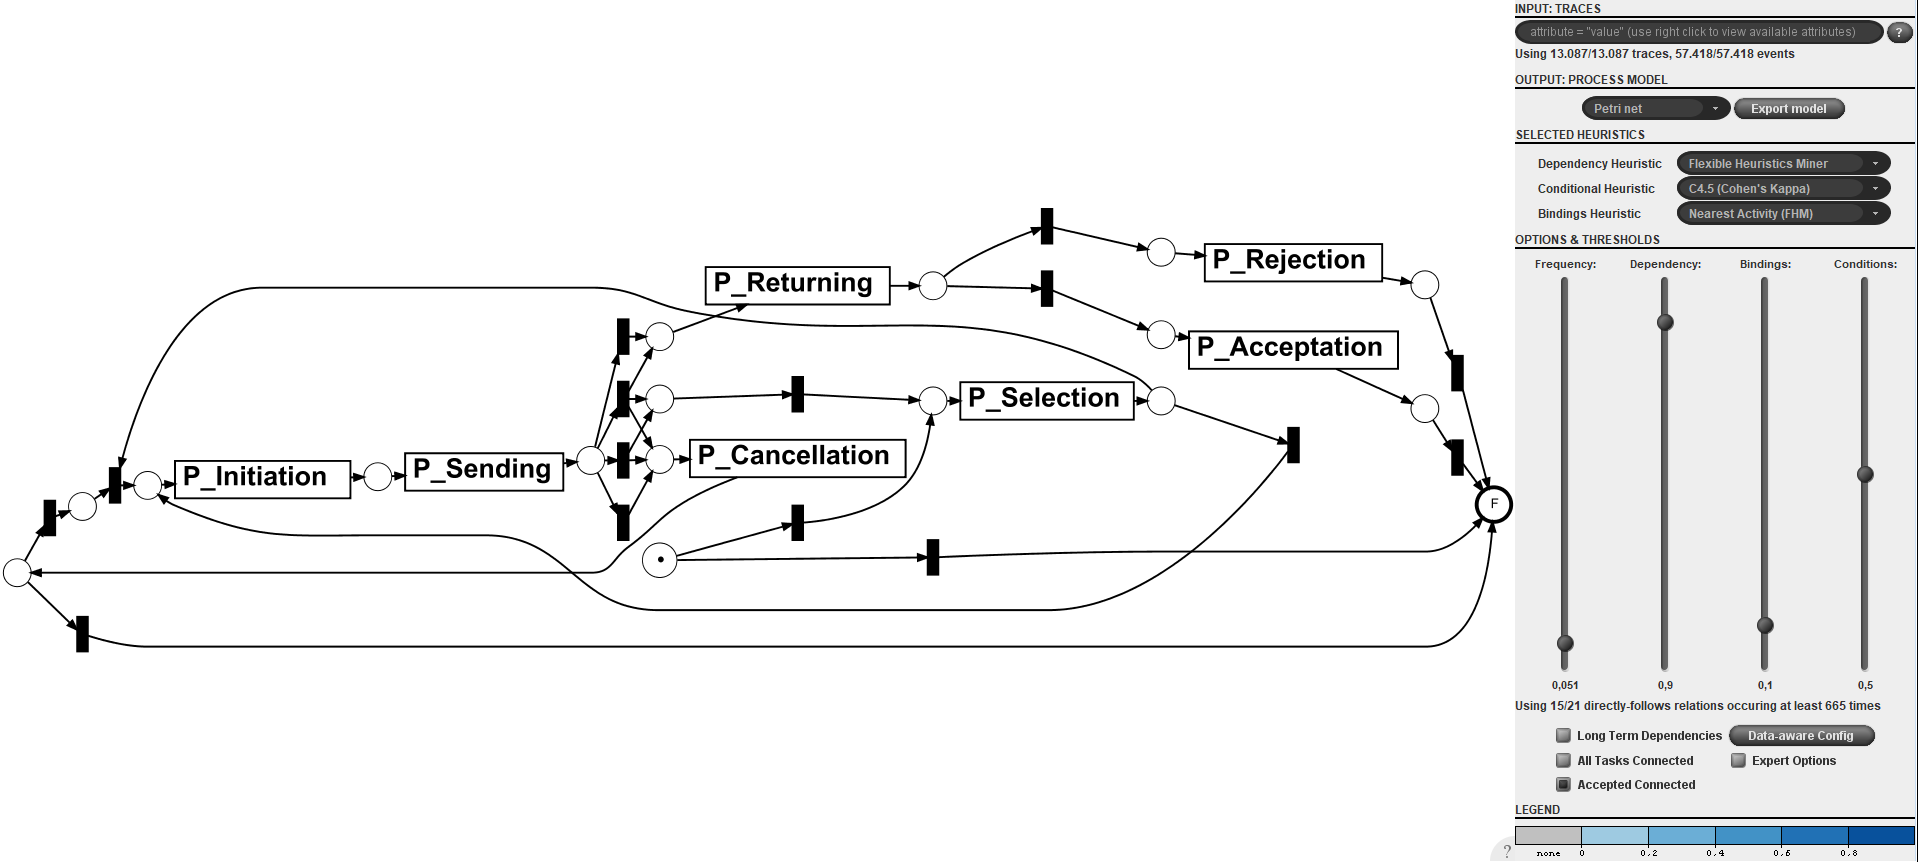
\includegraphics[width=\linewidth]{P_DirectlyFollowedFreq0-051.PNG}
  \caption{Directly followed graph 0.051 frequency filter}
  \label{fig:P_DFG0-051}
\end{subfigure}
\begin{subfigure}{.4\textwidth}
  \centering
  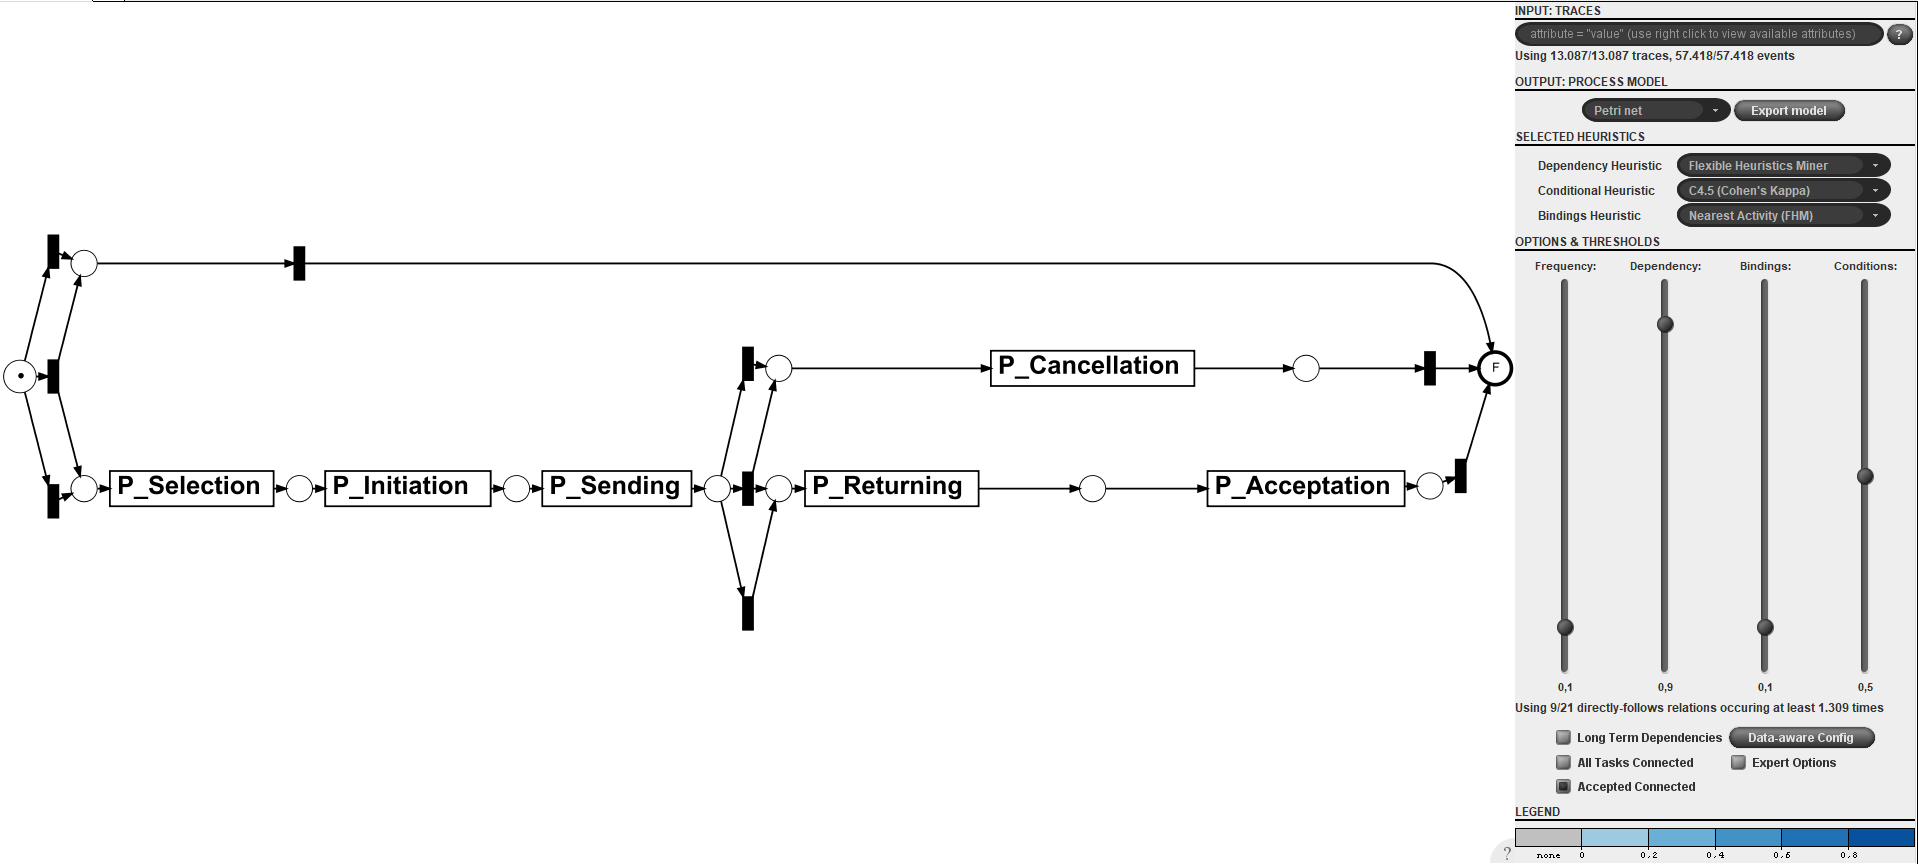
\includegraphics[width=\linewidth]{P_DirectlyFollowedFreq0-1.PNG}
  \caption{Petri net for 0.1 frequency filter}
  \label{fig:P_DFG0-1}
\end{subfigure}
\begin{subfigure}{.4\textwidth}
  \centering
  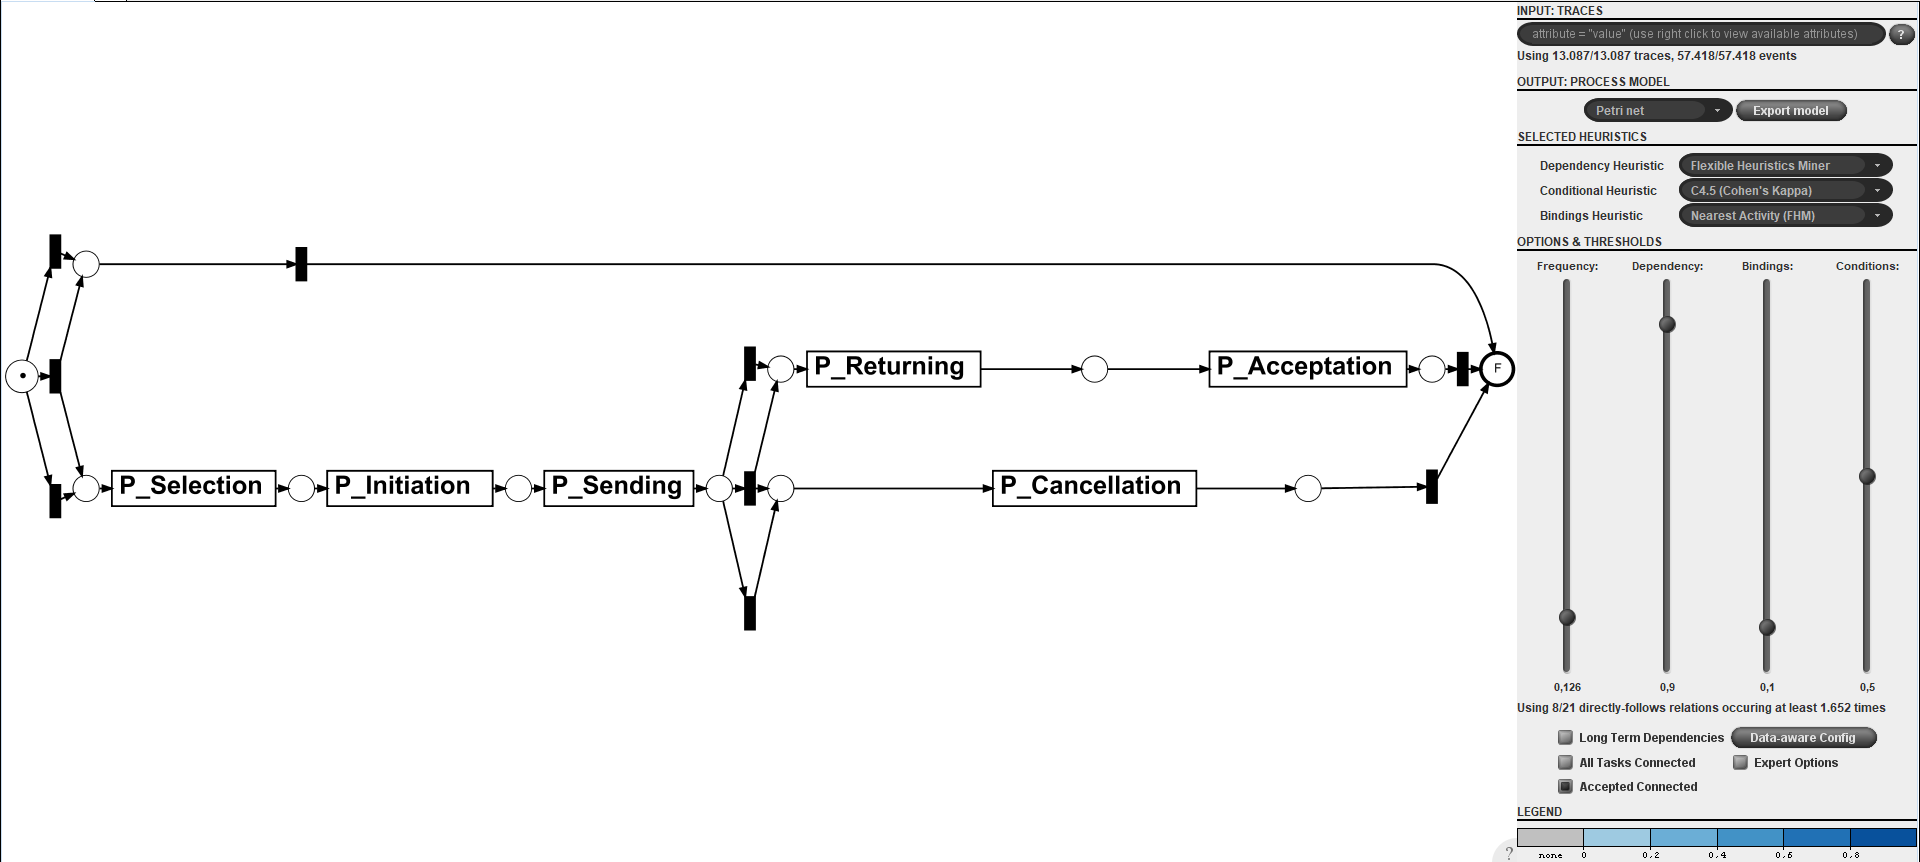
\includegraphics[width=\linewidth]{P_DirectlyFollowedFreq0-126.PNG}
  \caption{Petri net for 0.126 frequency filter}
  \label{fig:P_DFG0-126}
\end{subfigure}
\caption{Considered petri nets}
\label{fig:P_Direct}
\end{figure}

Because of simplicity reasons I picked out of those, figure \ref{fig:P_Direct}, just the 0.051 and 0.1 filtered petri nets and because of genralization not 0.126 or 0.2.


\begin{figure}[!htbp]
\centering
\begin{subfigure}{.4\textwidth}
  \centering
  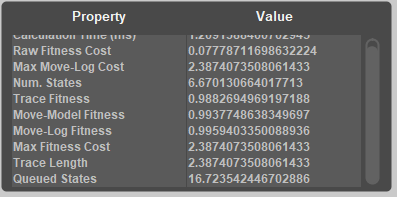
\includegraphics[width=\linewidth]{P_Conformance0-051.PNG}
  \caption{Conformance for 0.051 as frequency filter}
  \label{fig:P_Conf0-051}
\end{subfigure}%
\begin{subfigure}{.4\textwidth}
  \centering
  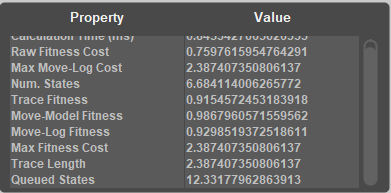
\includegraphics[width=\linewidth]{P_Conformance0-1.PNG}
  \caption{Conformance for 0.1 as frequency filter}
  \label{fig:P_Conf0-1}
\end{subfigure}
\begin{subfigure}{.4\textwidth}
  \centering
  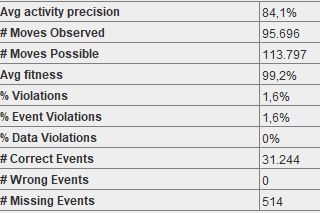
\includegraphics[width=\linewidth]{P_Precision0-051.PNG}
  \caption{Precision for 0.051 as frequency filter}
  \label{fig:P_Prec0-051}
\end{subfigure}%
\begin{subfigure}{.4\textwidth}
  \centering
  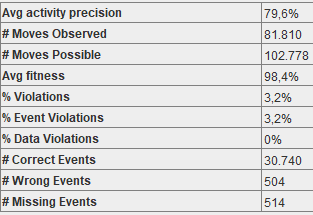
\includegraphics[width=\linewidth]{P_Precision0-1.PNG}
  \caption{Precision for 0.1 as frequency filter}
  \label{fig:P_Prec0-1}
\end{subfigure}
\caption{Conformance and precision checking}
\label{fig:P_ConfPrec}
\end{figure}


The conformance and precision outcomes, to see in figure \ref{fig:P_ConfPrec}, told me, that the 0.1 frequency model (fitness 91.55\%, precision 80\%) has not a good enough precision. And also the precision of the 0.051 filtered model is not really high. So I searched for an other model, which has a similar simplicity as the 0.1 and 0.051 filtered models and has maybe a better performance. The models fullfilling the simplicity criterium had 0.08 or 0.025 frequency filtered.

\begin{figure}[!htbp]
\centering
\begin{subfigure}{0.49\textwidth}
  \centering
  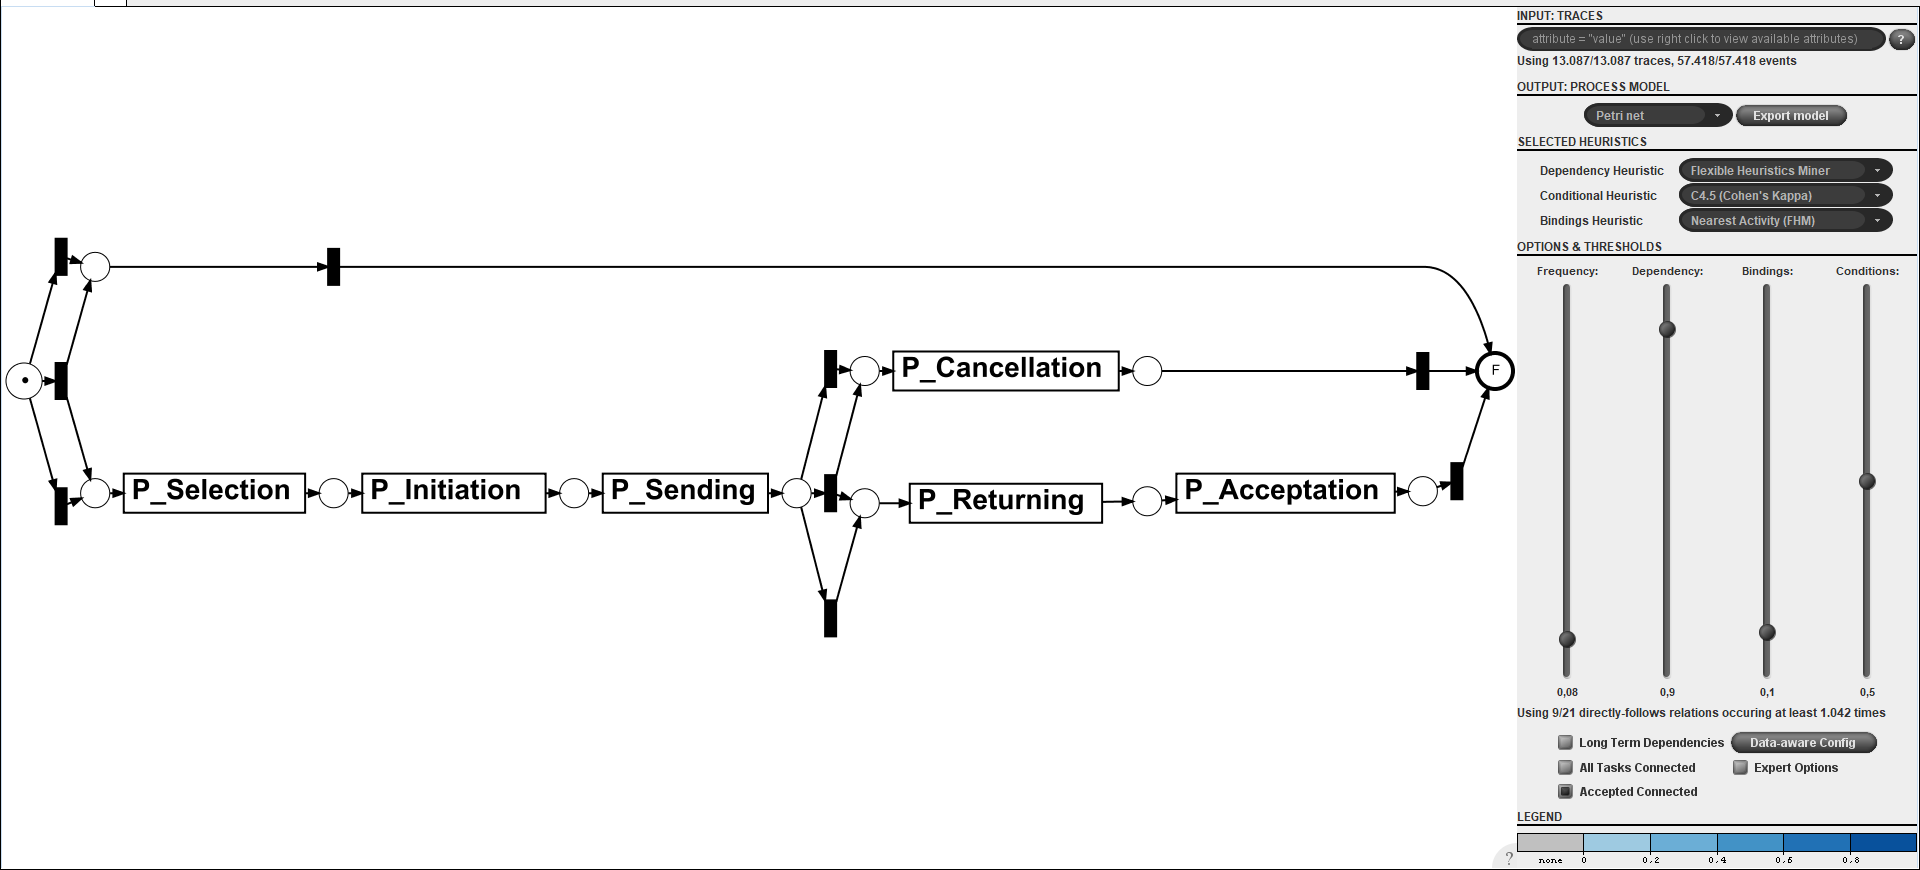
\includegraphics[width=0.8\linewidth]{P_DirectlyFollowedFreq0-08.PNG}
  \caption{0.08 frequency}
  \label{fig:P_0-08}
\end{subfigure}
\begin{subfigure}{0.49\textwidth}
  \centering
  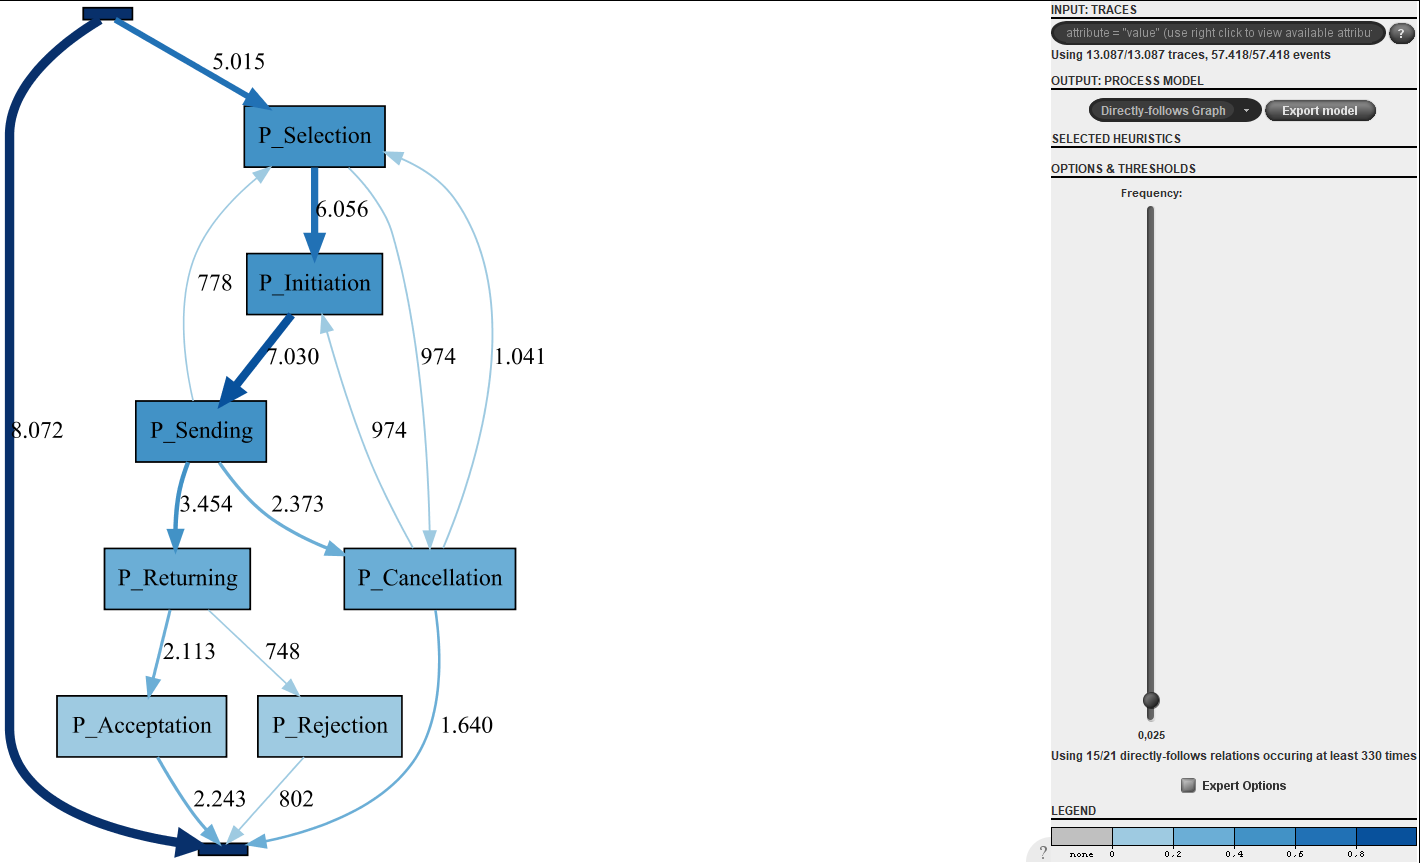
\includegraphics[width=0.8\linewidth]{P_DirectlyFollowedFreq0-025.PNG}
  \label{fig:P_0-025}
\end{subfigure}
\caption{Petri net}
\label{fig:P_Direct2Petri}
\end{figure}


\begin{figure}[!htbp]
\centering
\begin{subfigure}{0.4\textwidth}
  \centering
  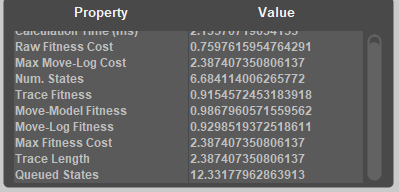
\includegraphics[width=\linewidth]{P_Conformance0-08.PNG}
  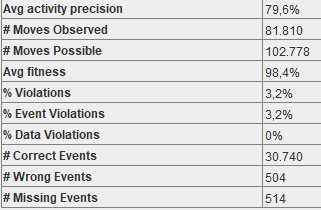
\includegraphics[width=1\linewidth]{P_Precision0-08.PNG}
  \caption{0.08 frequency}
  \label{fig:P_0-08}
\end{subfigure}
\begin{subfigure}{0.4\textwidth}
  \centering
  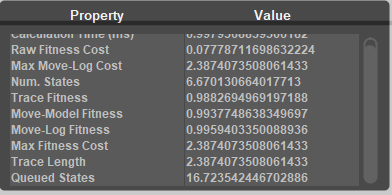
\includegraphics[width=1\linewidth]{P_Conformance0-025.PNG}
  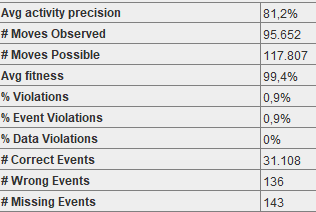
\includegraphics[width=\linewidth]{P_Precision0-025.PNG}
  \caption{0.025 frequency}
  \label{fig:P_0-025}
\end{subfigure}
\caption{Cnformance and precision}
\label{fig:P_Direct2}
\end{figure}

After having a look at all results in \ref{fig:P_Direct2} and comparing it with earlier results I chose the model with 0.051 frequency filter. The precision of 0.025 is with 83.6\% the same and the fitness is also the same, 98.82\%. With 0.08 filtering it had a worse fitness (91.54\%) and precision (80\%). All filtering inbetween were the same.


\subsubsection{Discussion of the lifecycle}
Simplifying the discussion I will not write "P\_.." in begin of all events, but every event mentioned in this section is from the proposal data set.

\begin{figure}[!htbp]
  \begin{center}
    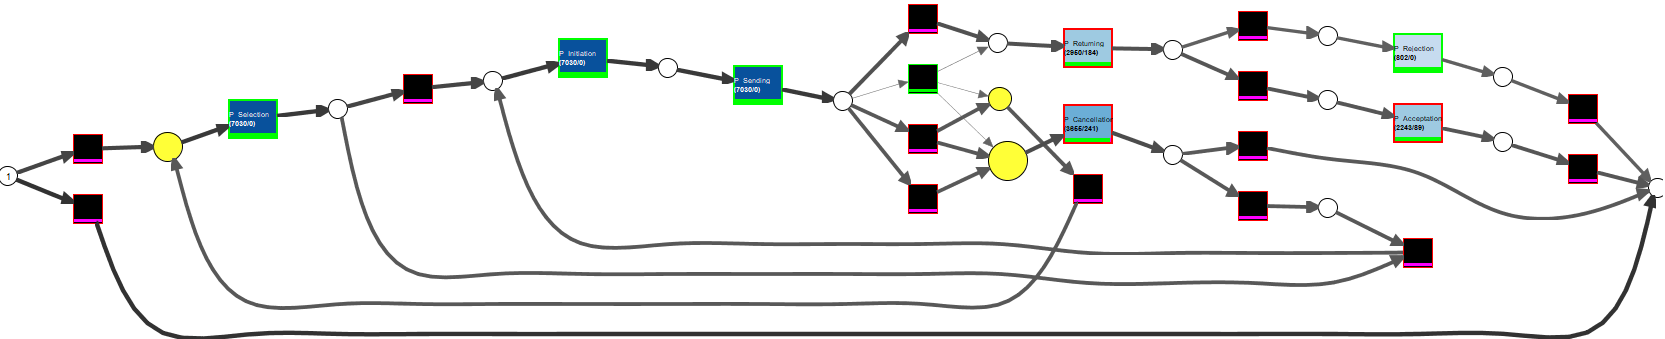
\includegraphics[width = 0.9\textwidth]{P_ConfomGraph0-051.png}
  \end{center}
  \caption{Replay on petri net with 0.051 frequency filter}
\end{figure}

This model has the conspicuousness, that 8072 cases directly end, but recheck it with the original graph this can be found, too. The other 5015 cases start with "Selection", which is executed in total 7030 times, because of a loop. Then "Initiation" event is performed (7030 cases), while in 2015 cases it also has to be executed "Cancellation" before  "Initiation" can be executed. "Initiation" is followed by "Sending" (7030 cases), which has 4 different succesor actions. 
\begin{enumerate}
	\item "Returning" (3143 cases, while in 184 cases a part of the trace is not to see in the model)
	\item "Returning", "Selection" and "Cancellation" (0 times)
	\item "Selection" and "Cancellation" (2015 times)
	\item "Cancellation"  (1881 times)
\end{enumerate}
"Returning" is in 802 cases followed by "Rejection" and in 2243 cases by "Acceptation". "Cancellation" is in 1881 cases the last action or it leads to "Initiation" (2015 times).

So there are two backloops to see in this model, which are executed in at most 25\% of the traces.

Furthermore are there 

\subsection{Combinded Model}
%Models that combine these two models into one showing the lifecycle of the application and the proposal together. Due to the high variability, you should discover one different model for each possible outcome, namely whether the application is finally rejected, cancelled or approved. 

For combinded Models I first filtered the data to have a dataset with all proposal data combined with the application data. This data I filtered with Heuristic filter (all configurations to 100\% and just deciding what the endstate is) with the outcomes/endstates "APP\_rejected" or "APP\_cancelled" or "APP\_approved". I saved them under the names "Filtered P App with approv", "Filtered P App with canc" and "Filtered P App with rej". 

\subsubsection{Endstate APP\_Approved}

\textbf{General Details of the data set}

The data set is collected between 1st of 0ct 2011 (saturday), 12:36:08 and 14th of Mar 2012 (Wednesday), 15:23:32. The set contains 301 and 4550 events executed. 

\begin{figure}[!htbp]
\centering
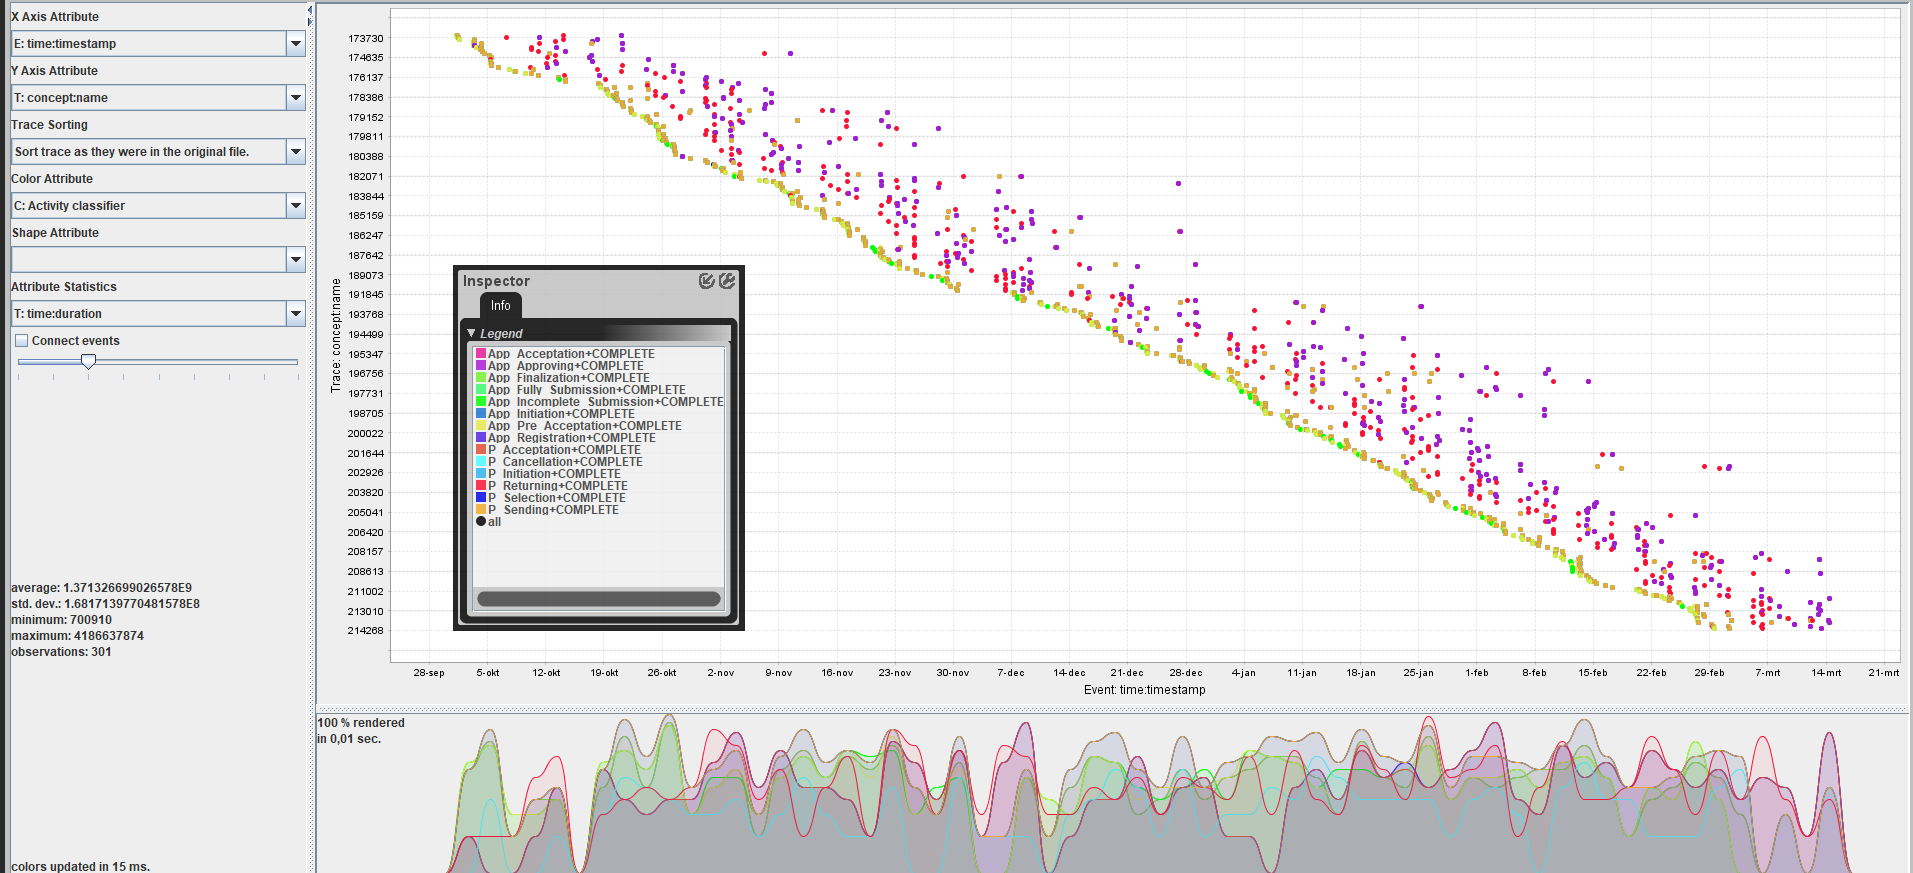
\includegraphics[height = 0.2\textheight]{ApprovalDot.PNG}
\caption{Dotted chart showing the time of events}
\label{fig:ApprovTimeFlow}
\end{figure}

In figure \ref{fig:ApprovTimeFlow} the dotted chart can be seen. There is a gap to see on every sunday. This is more clearly to see, when changing the color to days of the week. There you can see, that it is always a sunday. Furthermore is in the left below corner to see what the average duration of a case is, 15 days 20 hours 55 minutes and 26.70 seconds, and the maximum duration, 48 days 27 hours 23 minutes and 14.69 seconds. Both is given in milliseconds in the figure.

There are 14 different events:
"P\_Initiation" (10.0\%), "P\_Sending" (10.0\%), "P\_Selection" (10.0\%), "P\_Returning" (7.099\%), "App\_Pre\_Acceptation" (6.615\%), "App\_Initiation" (6.615\%), "App\_Approving" (6.615\%), "App\_Registration" (6.615\%), "App\_Finalization" (6.615\%), "App\_Fully\_Submission" (6.615\%), "App\_Incomplete\_Submission" (6.615\%), "App\_Acceptation" (6.615\%), "P\_Acceptation" (6.593\%), "P\_Cancellation" (3.385\%). The percentages are the relative occurences.
There are 73 different variants of traces.

Maximal 34 events are executed in a case and minimal 12. The mean of events per class is 15.116.


\textbf{Discover and evaluate models of lifecycle with Endstate APP\_Approved}

Like for approved and proposal I first checked different frequency filter setting to have a first idea, which models fullfill simplicity. Then for every chosen frequency in begin I checked conformance and precision.

\begin{figure}[!htbp]
\centering
\begin{tabular}{c|c|c|c|c|}
\cline{2-5}
& \multicolumn{4}{ c| }{Frequency} \\ \cline{2-5}
& 0 & 0.1 & 0.2 & 0.3 \\ \cline{1-5}
\multicolumn{1}{ |c|  }{Simplicity} 
& - & - & + & ++      \\ \cline{1-5}
\multicolumn{1}{ |c|  }{Fitness}  & 99.84 & 99.47 & 93.93 & 93.93      \\ \cline{1-5}
\multicolumn{1}{ |c| } {Precision} & 93.3 & 94.5 & 91.7 & 94.8  \\ \cline{1-5}
\end{tabular}
\caption{Results for approved as endstate}
\label{tab:ApprovRe}
\end{figure}

Based on the results, \ref{tab:ApprovRe}, I chose the model with 0.3 filtering. This one has a high simplicity, but still has surprisingly good results.
%TODO Maybe all together

\textbf{Discussion of the model}

\begin{figure}[!htbp]
\centering
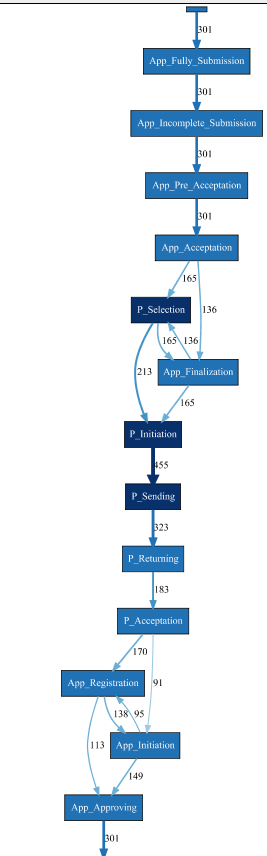
\includegraphics[width =0.9\textwidth]{APP_ApprovedDFG0-3.PNG}  
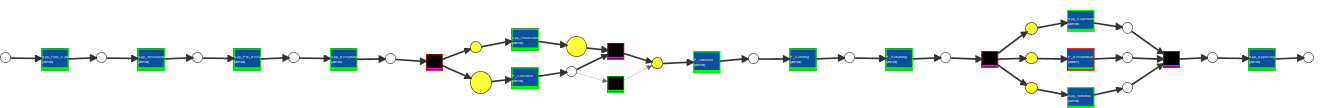
\includegraphics[width =0.9\textwidth]{ApprovReplay.PNG}
\caption{Endstate APP\_Approved}
\label{fig:ApprovModel}
\end{figure}

In figure \ref{fig:ApprovModel} the petri net and the result of the replat can be seen. It is hard to clearly read the details, but I describe it in detail here. 

All 301 cases start with the same 4 events: "App\_Fully\_Submission" \textrightarrow "App\_Incomplete\_Submission" \textrightarrow "App\_Pre\_Acceptation" \textrightarrow "App\_Acceptation". Then there are two events parallel: "App\_Finalization" and "P\_Selection". Before and after those actions are events skipped in the model, that occur in the original log. Afterwards "P\_Initiation" \textrightarrow "P\_Sending" \textrightarrow "P\_Returning" are executed in all cases. Again 3 events are parallel "App\_Registration", "App\_Registration" (just in 300 cases and "App\_Initiation". The last event is "App\_Approving".

When I controlled the time matrix for the transitions I saw, that there are a lot of transitions taking between 12 and 16 days.

\subsubsection{Endstate APP\_Cancelled}


\textbf{General Details of the data set}

The data set is collected between 1st of 0ct 2011 (saturday), 09:45:25 and 14th of Mar 2012 (Wednesday), 15:30:47. The set contains 1937 and 13524 events executed. 

\begin{figure}[!htbp]
\centering
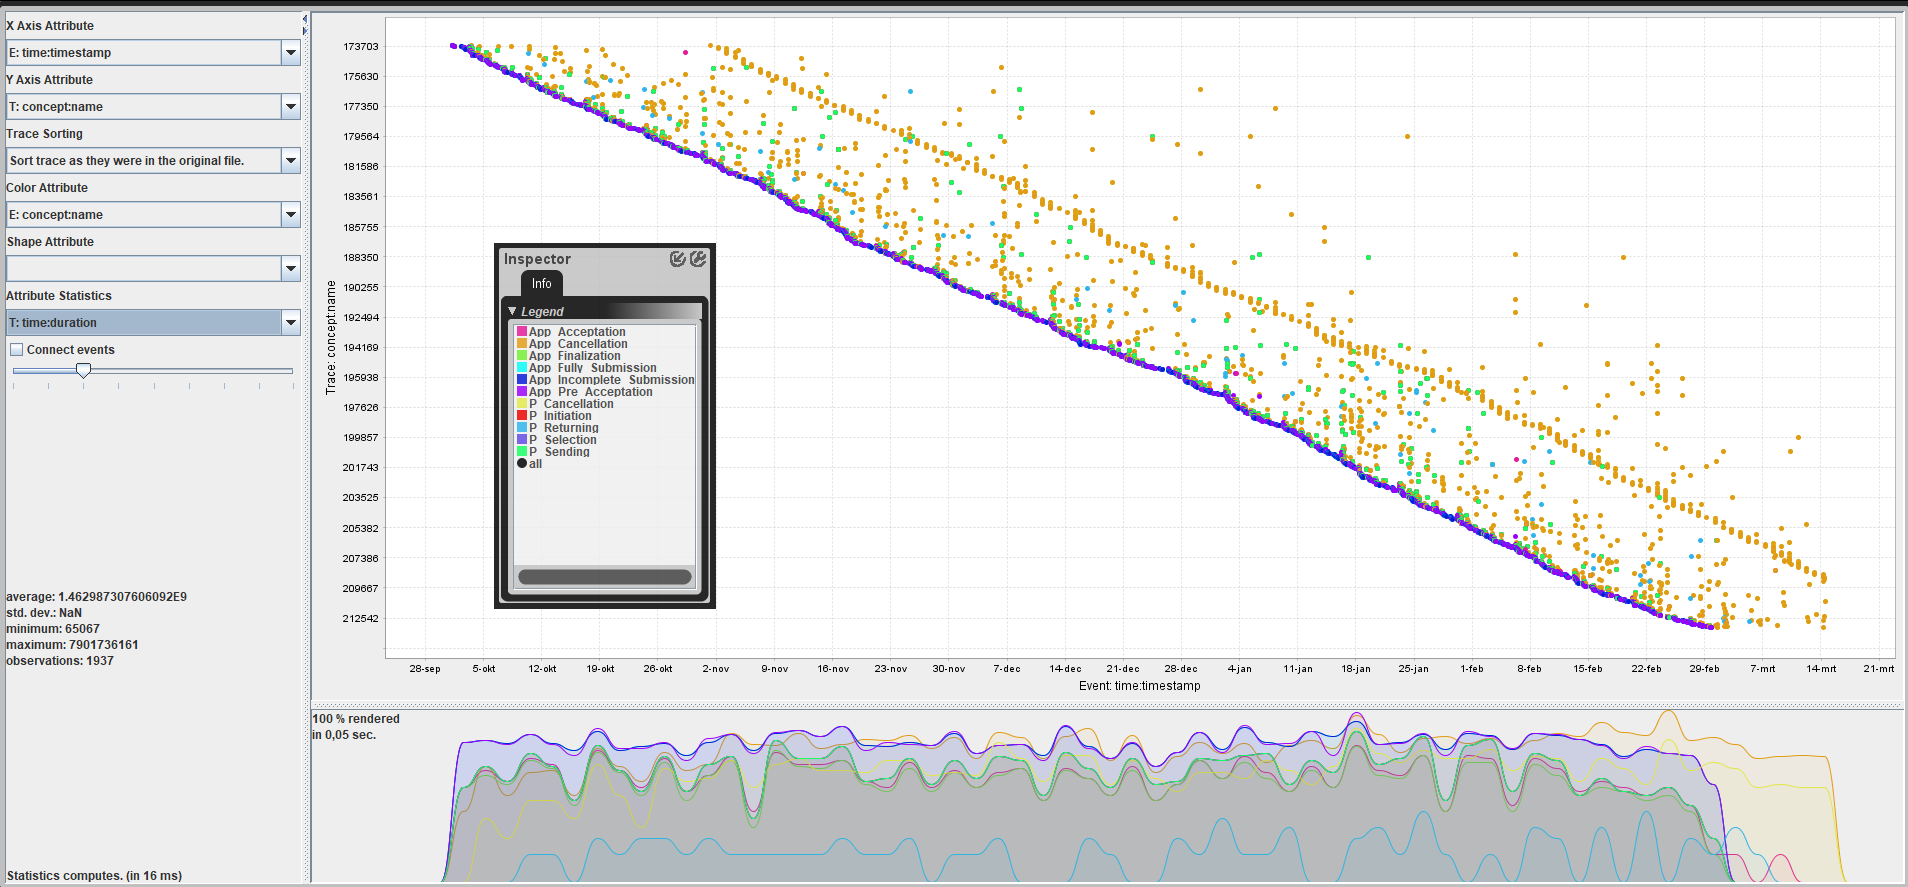
\includegraphics[height = 0.2\textheight]{CancDot.PNG}
\caption{Dotted chart showing the time of events}
\label{fig:CancTimeFlow}
\end{figure}

In figure \ref{fig:CancTimeFlow} the dotted chart can be seen. On every sunday there are just two events executed "App\_Pre\_Acceptation" and "App\_Incomplete\_Submission". Furthermore is in the left below corner to see what the average duration of a case is, 16 days 22 hours 23 minutes and 7.31 seconds, and the maximum duration, 90 days 3 hours 48 minutes and 38.29 seconds. Both is given in milliseconds in the figure.

There are 11 different events (relative occurences):
"App\_Cancellation" (14.323\%), "App\_Fully\_Submission" (14.323\%), "App\_Incomplete\_Submission" (14.323\%), "App\_Pre\_Acceptation" (14.315\%), "P\_Cancellation" (7.572\%), "P\_Initiation" (7.572\%), "P\_Sending" (7.572\%), "P\_Selection" (7.572\%), "App\_Acceptation" (6.182\%), "App\_Finalization" (5.694\%) and "P\_Returning" (0.555\%). There are 46 different variants of traces.

Maximal 32 events are executed in a case and minimal 3. The mean of events per class is 6.982.


\textbf{Discover and evaluate models of lifecycle with Endstate APP\_Cancelled}

\begin{figure}[!htbp]
\centering
\begin{tabular}{c|c|c|c|}
\cline{2-4}
& \multicolumn{3}{ c| }{Frequency} \\ \cline{2-4}
& 0 & 0.049 & 0.1 \\ \cline{1-4}
\multicolumn{1}{ |c|  }{Simplicity} 
& - & + & ++      \\ \cline{1-4}
\multicolumn{1}{ |c|  }{Fitness}  & 99.96 & 99.39 & 96.84       \\ \cline{1-4}
\multicolumn{1}{ |c| } {Precision} & 92.5 & 91.8 & 94.6   \\ \cline{1-4}
\end{tabular}
\caption{Results for cancelled as endstate}
\label{tab:CancRe}
\end{figure}
Like for APP\_Approved I checked different configurations and based on the results, \ref{tab:CancRe}, I decided to pick 0.1 filtered frequency model. The fitness and precision is still higher than 90\%, but it is also the most simpel model.

\textbf{Discussion of the model}

\begin{figure}[!htbp]
\centering
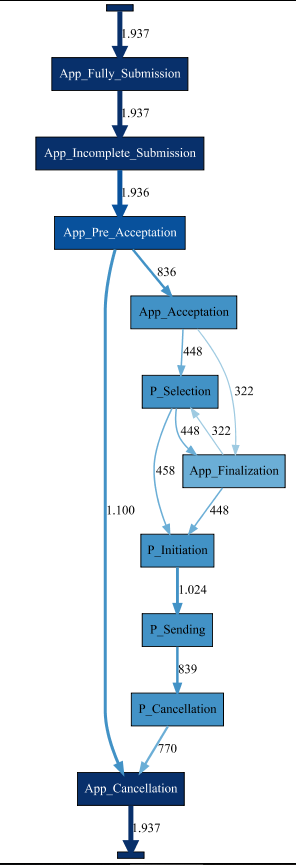
\includegraphics[width=0.9\textwidth]{APP_CancDFG0-1.PNG}
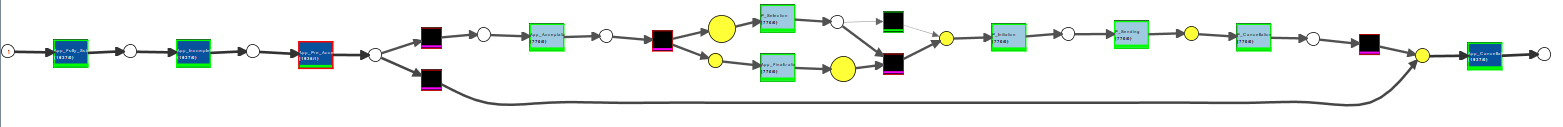
\includegraphics[width=0.9\textwidth]{CancReplay.PNG}
\caption{Endstate APP\_Cancelled}
\label{fig:CancModel}
\end{figure}

In figure \ref{fig:CancModel} the petri net and the result of the replat can be seen.

All cases start with "App\_Fully\_Submission" \textrightarrow "App\_Incomplete\_Submission" \textrightarrow "App\_Pre\_Acceptation" (this is just executed in 1936 cases). Then in 1167 cases "App\_Cancellation" follows directly. Otherwise "App\_Acceptation" (770 cases), followed by "P\_Selection" and "App\_Finalization", but those both can appear in both orders. After those are executed, "P\_Initiation" \textrightarrow "P\_Sending" \textrightarrow "P\_Cancellation" \textrightarrow"App\_Cancellation" is executed.

The time transition matrix showed me, that the transition to "App\_Finalization" and "P\_Cancellation" took the most time (between 17 and 22.5 days).


\subsubsection{Endstate APP\_Rejected}

\textbf{General Details of the data set}

The data set is collected between 1st of 0ct 2011 (saturday), 08:11:08 and 14th of Mar 2012 (Wednesday), 15:20:23. The set contains 7252 and 26691 events executed. 

\begin{figure}[!htbp]
\centering
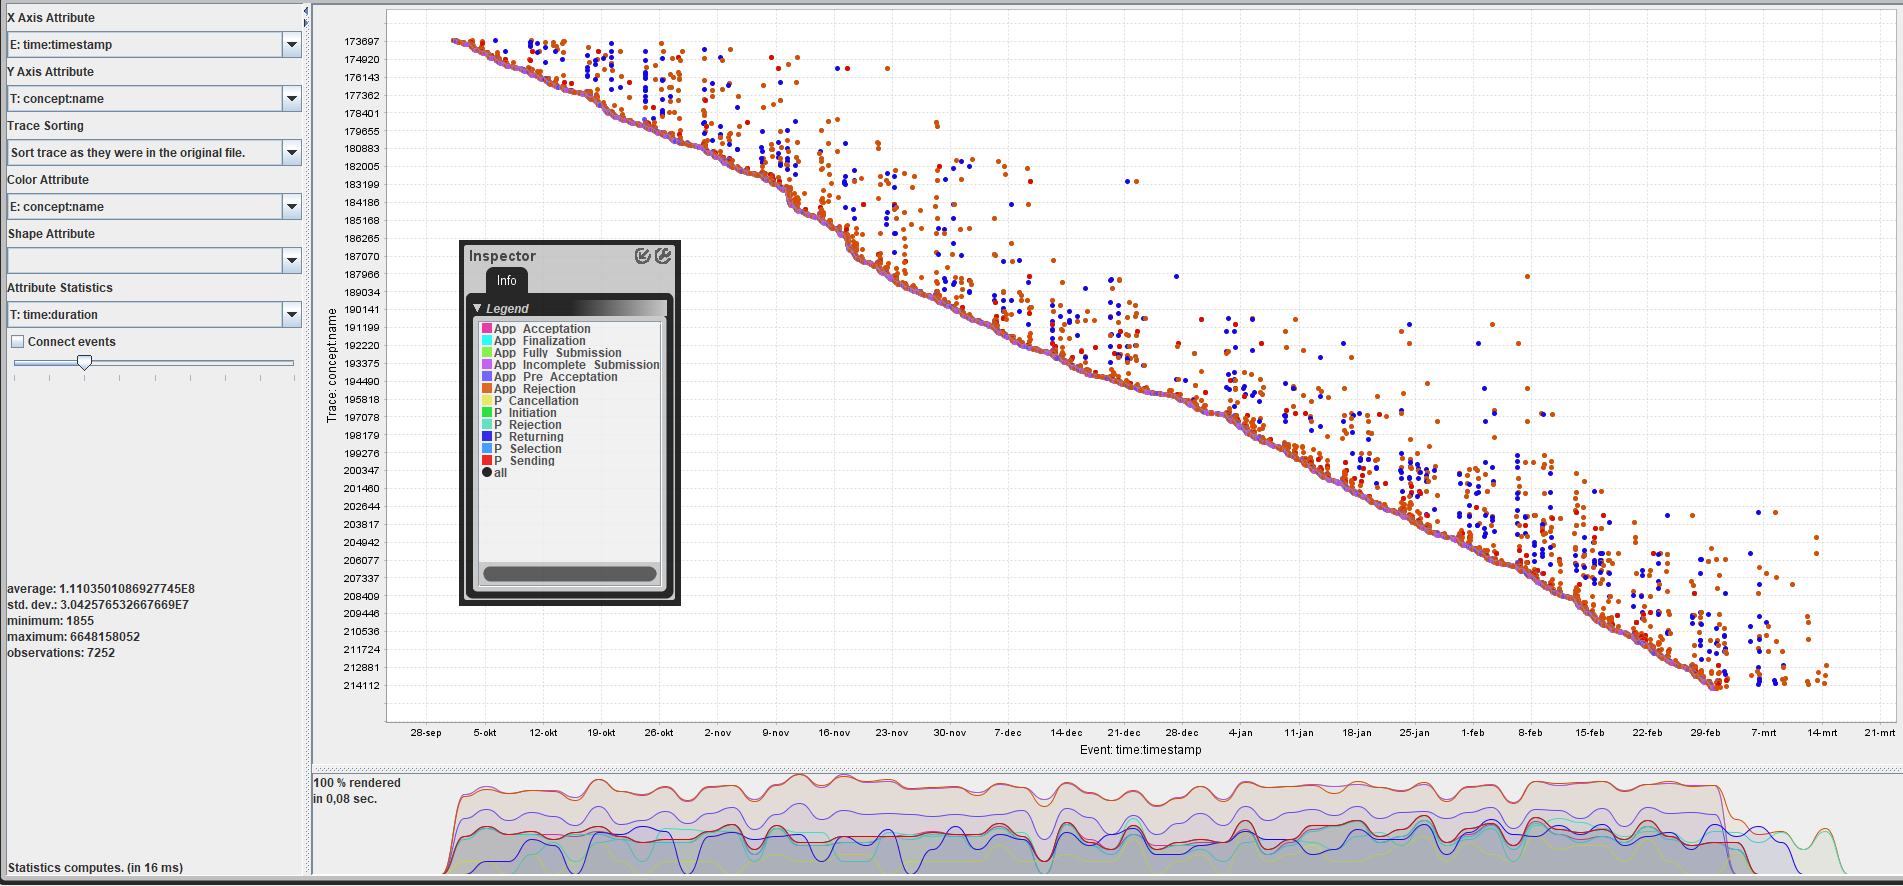
\includegraphics[height = 0.2\textheight]{RejDot.PNG}
\caption{Dotted chart showing the time of events}
\label{fig:RejTimeFlow}
\end{figure}

In figure \ref{fig:RejTimeFlow} the dotted chart can be seen. On every sunday there are just two events executed "App\_Rejection" and "App\_Incomplete\_Submission". Furthermore is in the left below corner to see what the average duration of a case is, 1 days 6 hours 50 minutes and 35.01 seconds, and the maximum duration, 76 days 22 hours 42 minutes and 38.05 seconds. Both is given in milliseconds in the figure.

There are 12 different events (relative occurences):
"App\_Rejection" (27.17\%), "App\_Fully\_Submission" (27.17\%), "App\_Incomplete\_Submission" (27.17\%), "App\_Pre\_Acceptation" (5.744\%), "P\_Initiation" (1.997\%), "P\_Sending" (1.997\%), "P\_Selection" (1.997\%), "App\_Acceptation" (1.678\%), "App\_Finalization" (1.57\%), "P\_Rejection" (1.57\%), "P\_Returning" (1.51\%), "P\_Cancellation" (0.427\%). There are 30 different variants of traces.

Maximal 12 events are executed in a case and minimal 3. The mean of events per class is 3.681.


\textbf{Discover and evaluate models of lifecycle with Endstate APP\_Rejected}

The last analysis is of the models ending in APP\_Rejected. In the first step I checked different frequency filters and decided based on simplicity and traceability I had a closer look at 0, 0.025 and 0.1.

\begin{figure}[!htbp]
\centering
\begin{tabular}{c|c|c|c|}
\cline{2-4}
& \multicolumn{3}{ c| }{Frequency} \\ \cline{2-4}
& 0 & 0.025 & 0.1 \\ \cline{1-4}
\multicolumn{1}{ |c|  }{Simplicity} 
& - & + & +++      \\ \cline{1-4}
\multicolumn{1}{ |c|  }{Fitness}  & 1.00 & 99.60 & 96.91       \\ \cline{1-4}
\multicolumn{1}{ |c| } {Precision} & 99.3 & 98.7 & 100   \\ \cline{1-4}
\end{tabular}
\caption{Results for cancelled as endstate}
\label{tab:RejRe}
\end{figure}

Based on \ref{tab:RejRe} I chose 0.1 filtered frequency model as the best. It is really easy to follow and has a good fitness.

\textbf{Discussion of the model}

\begin{figure}[!htbp]
\centering
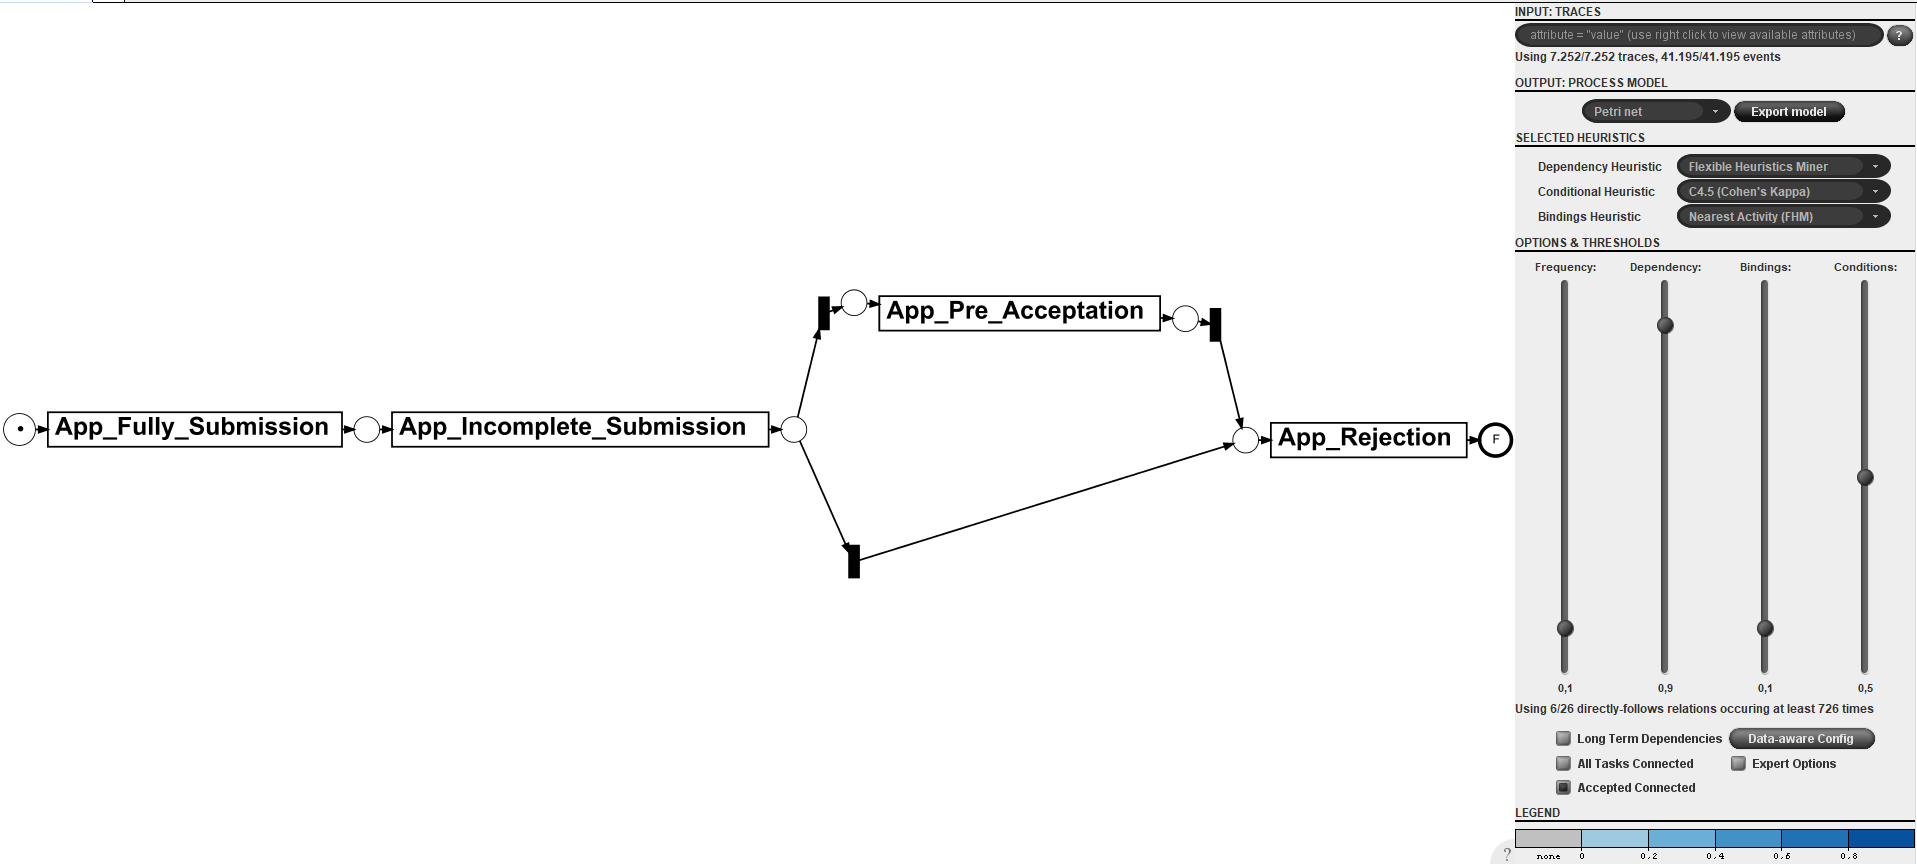
\includegraphics[width=0.9\textwidth]{Rej0-1.PNG}
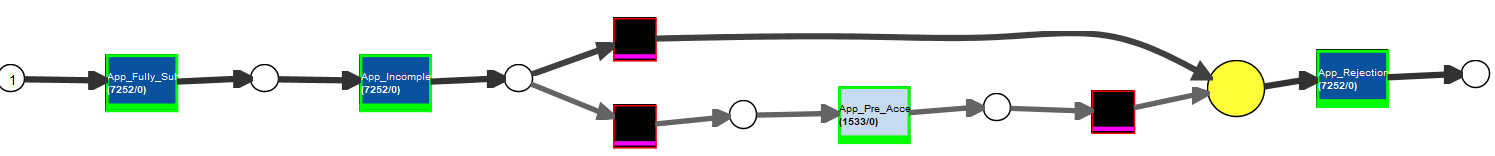
\includegraphics[width=0.9\textwidth]{RejReplay.PNG}
\caption{Endstate APP\_Rejected}
\label{fig:RejModel}
\end{figure}

In figure \ref{fig:RejModel} the model and the replay can be seen. 

The process starts with "App\_Fully\_Submission" \textrightarrow "App\_Incomplete\_Submission" (7252 cases). This is or followed directly by "App\_Rejection" (5719 cases) or first by "App\_Pre\_Acceptation" (1533 cases) and then "App\_Rejection". There are for "App\_Rejection" details not presented in the model because of the filtering.

The worst transition is with 5.51 days from "App\_Pre\_Acceptation" to "App\_Rejection".

\subsection{C-net of the proposal process}
%Analyze the C-net of the proposal process and explain it. 

Based on the results of my analysis of the model before I chose the same frequency filtering for the C-net of the proposal process.
\begin{figure}[!htbp]
\centering
\begin{subfigure}{0.8\textwidth}
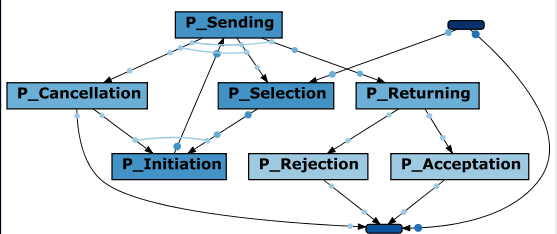
\includegraphics[height = 0.2\textheight]{PCnet0-05.PNG}
\caption{C-net with 0.051 filtered frequency}
\label{fig:cnetP0-025}
\end{subfigure}
\begin{subfigure}{0.8\textwidth}
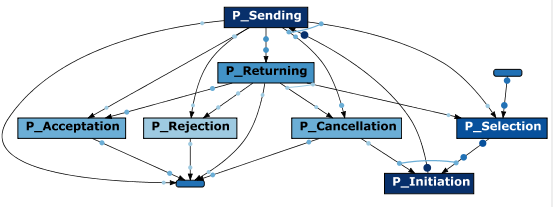
\includegraphics[height = 0.2\textheight]{PropC-Net0.PNG}
\caption{C-net without filtered frequency}
\label{fig:cnetP0}
\end{subfigure}
\caption{C-Nets of the proposal process}
\label{fig:cNetP}
\end{figure}

In \ref{fig:cNetP} I show two C-nets of the proposal process for comparsion. \ref{fig:cnetP0-025} is the one I picked and I will discuss in detail. In \ref{fig:cnetP0} the original C-net of the process is to see and obviously it is much more complicated and not so intuitive than the filtered one. 

\subsubsection{Analysis of the C-net}
For simplicity reasons I will not write "P\_" as prefix of every activity.

The first thing I did is having a look at the maximal number of bindings. This is for sending with 4 possible bindings. The input is always from initiation, but there are 4 different outputs possible.  Just checking the possible traces shows you, that there are infinite many possible traces, because of a loop between sending and initiation. All trace possibilities:
\begin{figure}[!htbp]
\begin{itemize}
	\item Done
	\item Selection \textrightarrow Initiation \textrightarrow Sending \textrightarrow
	\begin{itemize}
	\item  Returning \textrightarrow
	\begin{itemize}
		\item Acceptation \textrightarrow Done
		\item Rejection \textrightarrow Done
	\end{itemize}
	\item ((Cancellation \textrightarrow Selection) or (Selection \textrightarrow Cancellation)) \textrightarrow Initiation \textrightarrow Sending ...
	\item Cancellation \textrightarrow Done
	\end{itemize}
\end{itemize}
\end{figure}

This pathes are also what you would expect. The sending step has the biggest variance when looking at the succesor events and we have a fixed prefix for every case, that not directly ends.


\subsection{Own Petri net of the proposal process}
%Based on your analysis, create a Petri net of the proposal process by your own. For example, do not consider infrequent paths and also outlier behaviors. 


\subsection{Analysis of the performance of Application and work process}
%Analyze the performance of Application and work process. What are the bottlenecks? What are your recommendations to the company to increase the performance of the process? 

Just the events beginning with "P\_..." or "W\_..." are required. The resulting data set is saved as "Filtered Work and App".

\subsubsection{General Details of the data set}
The data set is collected between 1st of 0ct 2011 (saturday), 00:38:44 and 14th of Mar 2012 (Wednesday), 16:04:54 and contains 13087 cases with 230956 events. 

\begin{figure}[!htbp]
\centering
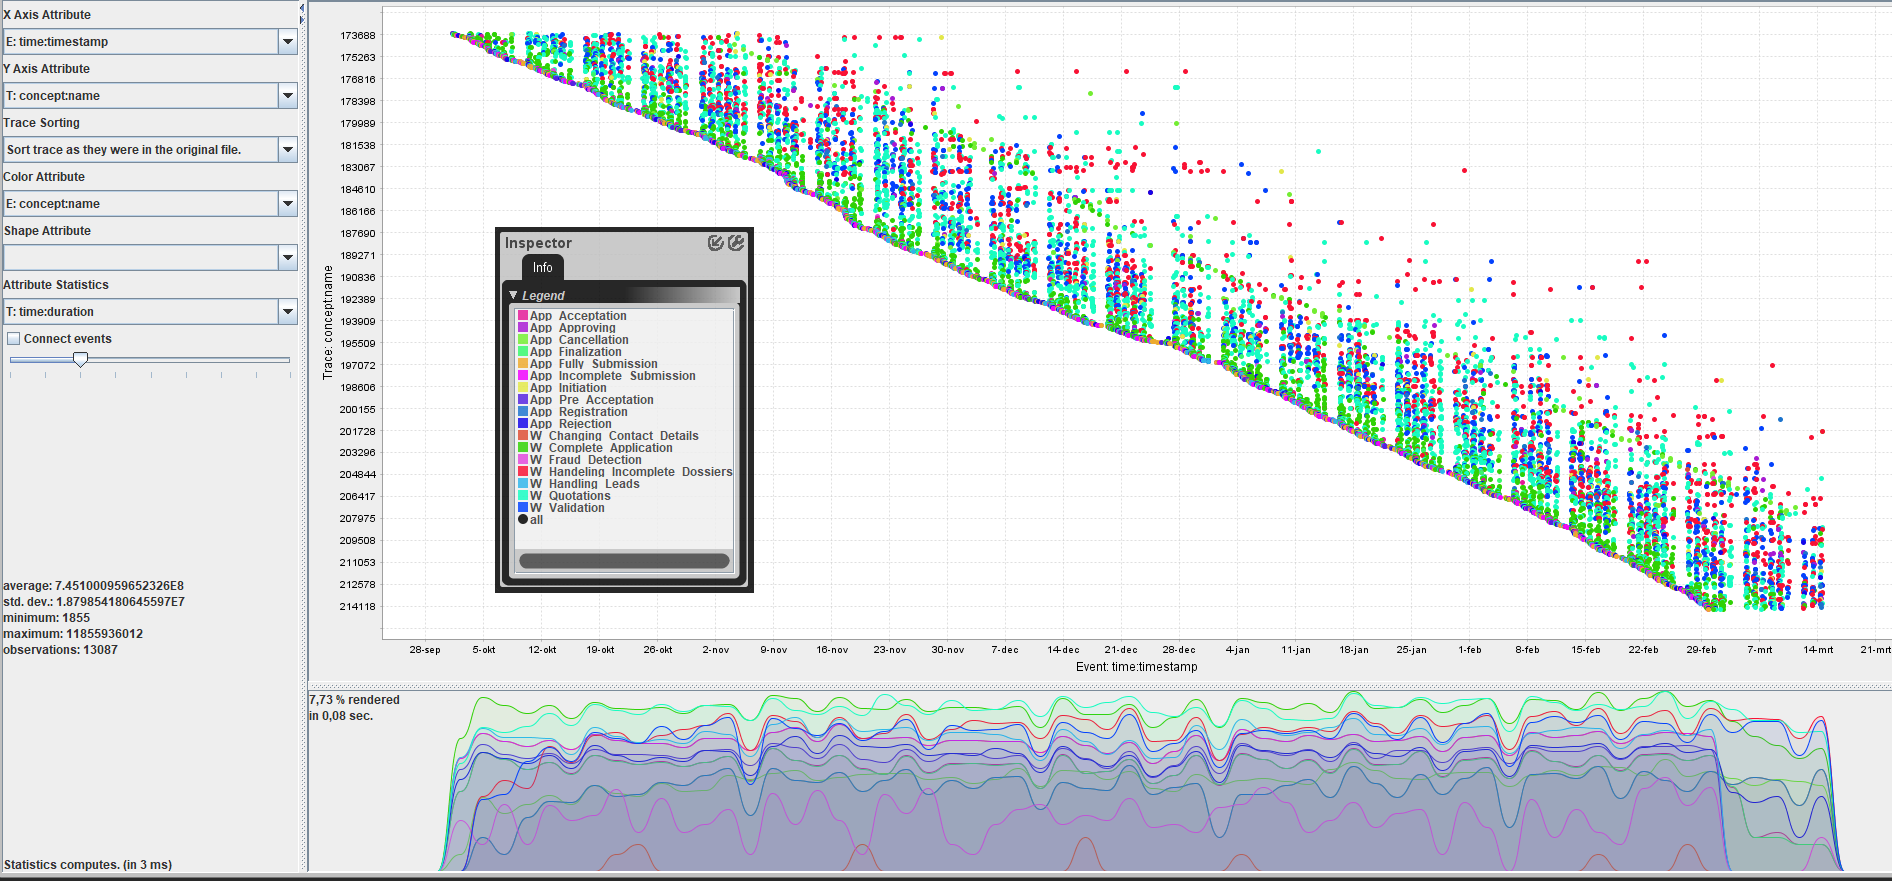
\includegraphics[width = 0.8\textwidth]{AppWorkDot.PNG}
\caption{Dotted chart showing the time of events}
\label{fig:AppWorkTimeFlow}
\end{figure}

In figure \ref{fig:AppWorkTimeFlow} the dotted chart can be seen. Having a closer look at this I saw again gaps on sunday. On sundays just "App\_Incomplete\_Submission" and "App\_Rejection" is been executed. Furthermore is in the left below corner to see what is the average duration of a case, 8 days 14 hours 58 minutes and 20.10 seconds, and the maximum duration, 137 days 5 hours 18 minutes and 56.01 seconds. Both is given in milliseconds.

The data set has 29 events (occurence relative): 
"W\_Complete\_Application" (10.377\%), "W\_Complete\_Application" (10.18\%), "W\_Quotations" (9.948\%), "W\_Quotations" (9.701\%), "App\_Fully\_Submission" (5.666\%), "App\_Incomplete\_Submission" (5.666\%), "W\_Handeling\_Incomplete\_Dossiers" (4.939\%), "W\_Handeling\_Incomplete\_Dossiers" (4.936\%), "W\_Validation" (3.418\%), "W\_Validation" (3.417\%), "App\_Rejection" (3.306\%), "W\_Complete\_Application" (3.192\%), "App\_Pre\_Acceptation" (3.19\%), "W\_Quotations" (2.872\%), "W\_Handling\_Leads" (2.554\%), "W\_Handling\_Leads" (2.553\%), "App\_Acceptation" (2.214\%), "W\_Validation" (2.175\%), "App\_Finalization" (2.171\%), "W\_Handling\_Leads" (2.066\%), "App\_Cancellation" (1.215\%), "W\_Handeling\_Incomplete\_Dossiers" (1.032\%), "App\_Initiation" (0.972\%), "App\_Approving" (0.972\%), "App\_Registration" (0.972\%), "W\_Fraud\_Detection" (0.117\%), "W\_Fraud\_Detection" (0.117\%), "W\_Fraud\_Detection" (0.054\%) and "W\_Changing\_Contact\_Details" (0.005\%).

There are 3668 different variants of traces.

Maximal 162 events are executed in a case and minimal 3. The mean of events per class is 17.648.

All cases start with "App\_Fully\_Submission", but there are 12 different outcomes: 
"App\_Rejection" (26.202\%), "W\_Validation" (20.975\%), "W\_Handling\_Leads" (17.07\%), "W\_Complete\_Application" (14.816\%), "W\_Quotations" (9.895\%), "App\_Cancellation" (7.091\%), "W\_Handeling\_Incomplete\_Dossiers" (3.454\%), "W\_Fraud\_Detection" (0.436\%), "W\_Changing\_Contact\_Details" (0.031\%), "W\_Validation" (0.015\%), "App\_Registration" (0.008\%) and "W\_Quotations" (0.008\%).